%-----------------------------------------------------------------------------%
\chapter{\babTiga}
\label{bab:3}
%-----------------------------------------------------------------------------%
Bab ini menjelaskan tentang hal-hal \f{advanced} dalam \gls{latex}.
Hal ini mencakup bagaimana cara menulis persamaan matematis di \gls{latex}, menambahkan daftar isi, catatan, \acrshort{pdf}, menambahkan kode, bahkan menambahkan perintah baru.

This chapter details the


%-----------------------------------------------------------------------------%
\section{Latviz}
\label{sec:Latviz}
%-----------------------------------------------------------------------------%
The visualization tool Latviz is a web application that provides visualizations for ML-KEM, ML-DSA, LLL, and BKZ algorithms, meant to help users more easily understand the four through interactive visualizations.

\subsection{Architecture}
Latviz is built using Next.js, a fullstack React-based framework, along with Tailwind CSS for the frontend and primarily Typescript for the backend processes. The ML-KEM and ML-DSA algorithms are implemented using a modification of an existing Javascript library ’pqc’ \cite{kalava} that allows for the display of the inner workings of both algorithms as opposed to only the outputs. The LLL and BKZ algorithms are implemented through a modification of lll-attack-runner \cite{6} that allows for the display of textual information relating to the algorithms, and are visualized using a combination of D3 and React.

\begin{figure}[H]
\centering
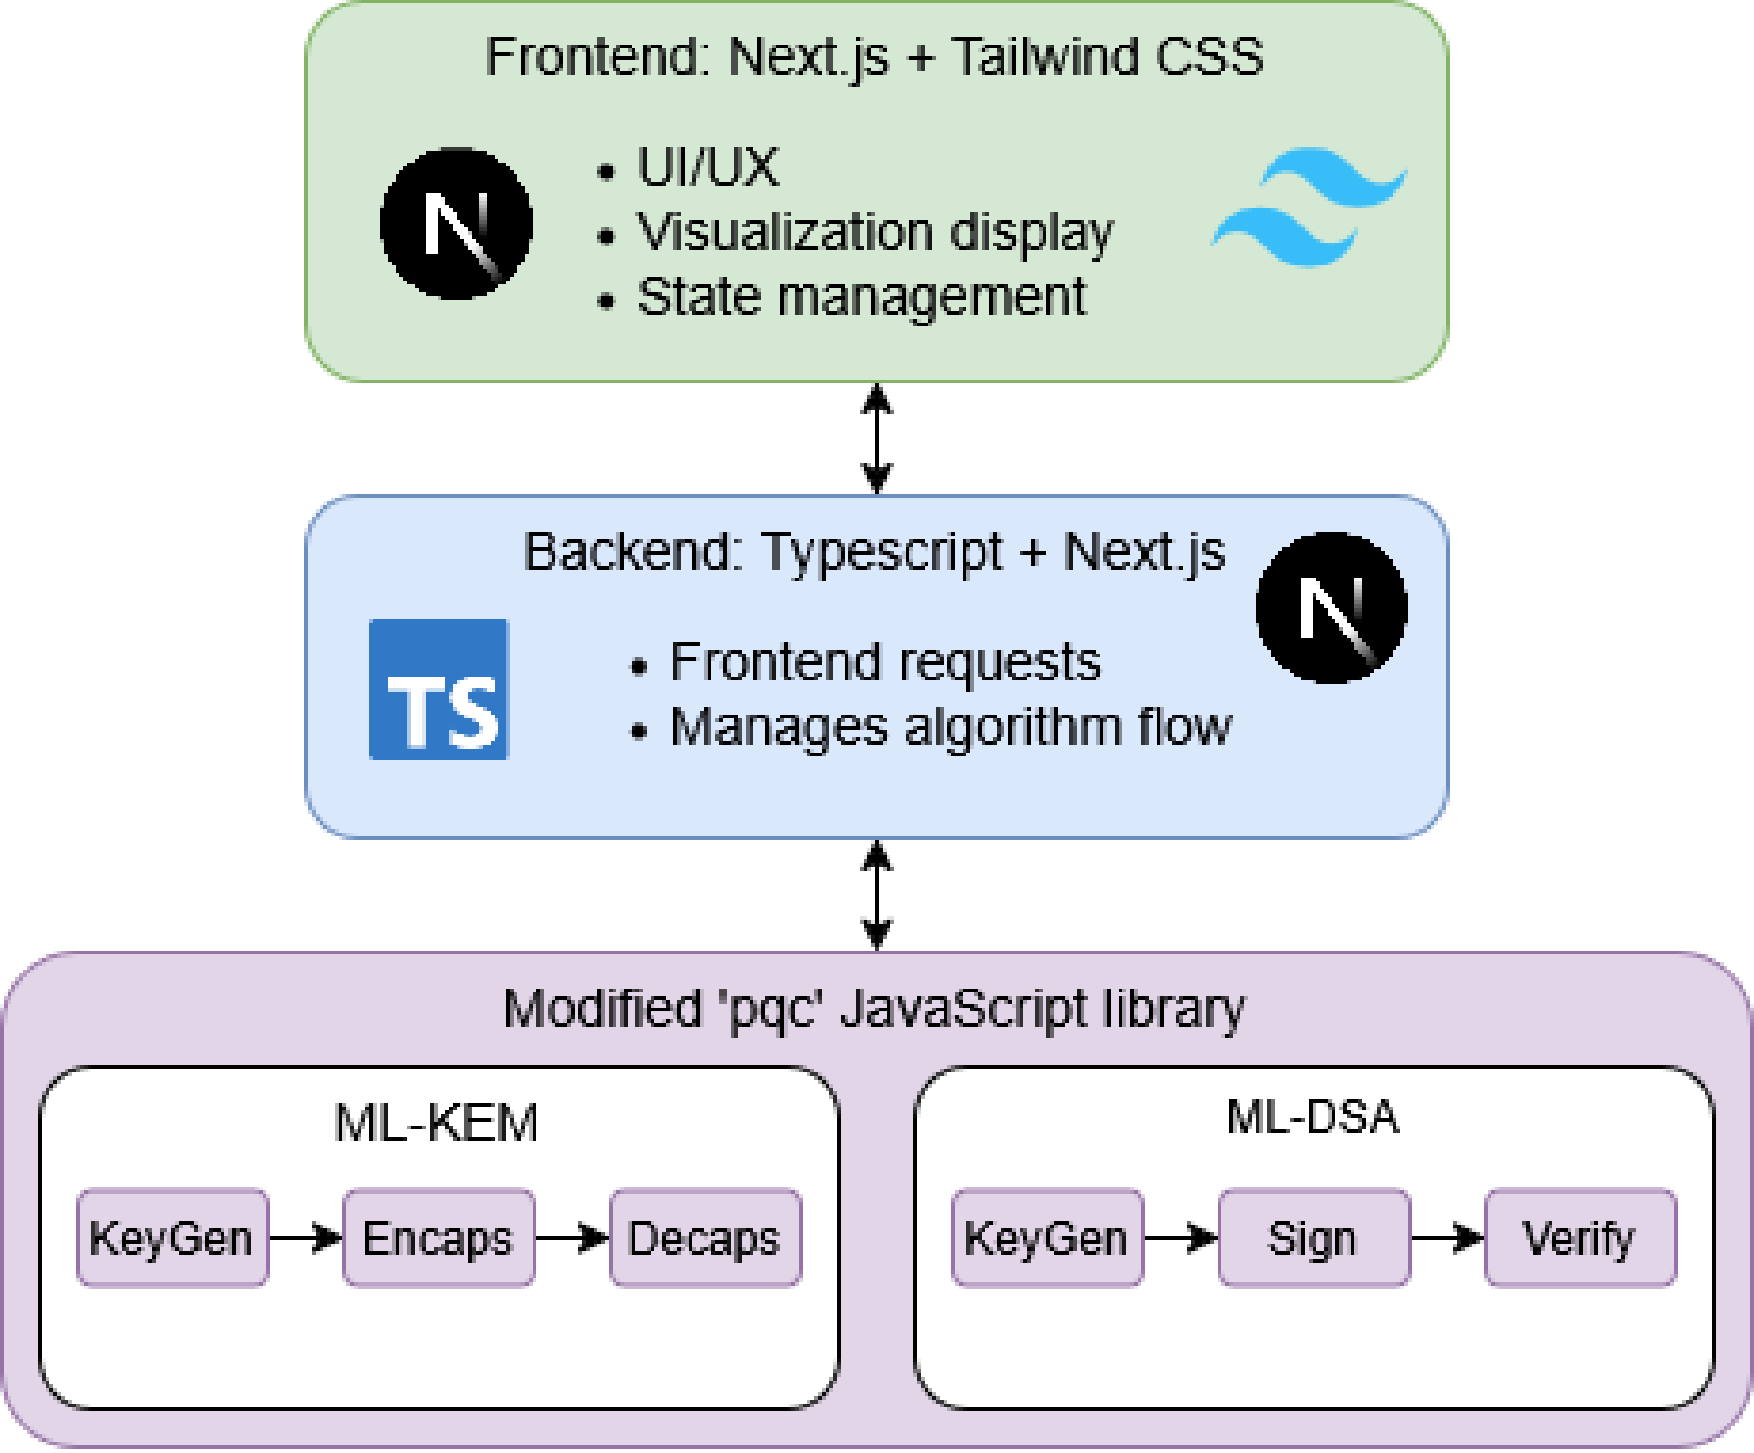
\includegraphics[width=.48\linewidth]{assets/pdfs/Architecture_diagram.pdf}
\caption{Architecture of Latviz's ML-KEM and ML-DSA visualization}
\label{fig10}
\end{figure}

\begin{figure}[H]
    \centering
    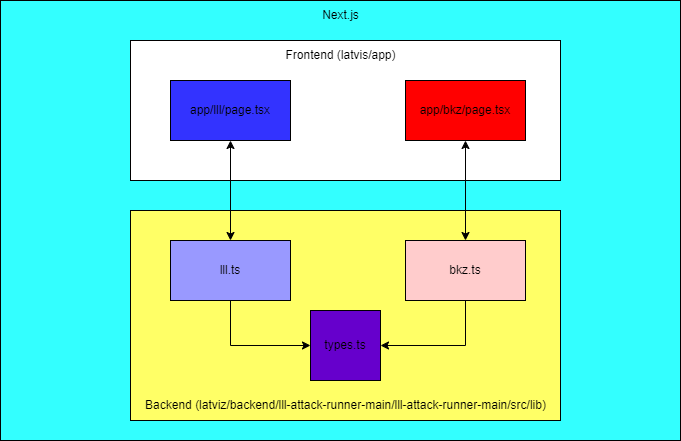
\includegraphics[width=0.7\textwidth]{assets/pics/appstructure.png}
    \caption{Program structure of Latviz's LLL and BKZ visualization}
    \label{Program diagram structure}
\end{figure}

\subsection{Visualization Structure}

\subsubsection{ML-KEM and ML-DSA}
The visualizations for both algorithms follow the same general structure. Both contain three main sections, starting with an about section at the top of the page, followed by a visualization of the scheme in use, and finally by a full visualization of an instance of the chosen algorithm. For the sake of brevity, this section will only be going into the page for ML-DSA, though both pages are structurally identical.
After opening the page for the algorithm, the first thing the user sees is a short explanation on the chosen algorithm; what it is, what it is set to replace, and what its difficulty is based on. Below is what the section looks like for ML-DSA:

\begin{figure}[H]
\centering
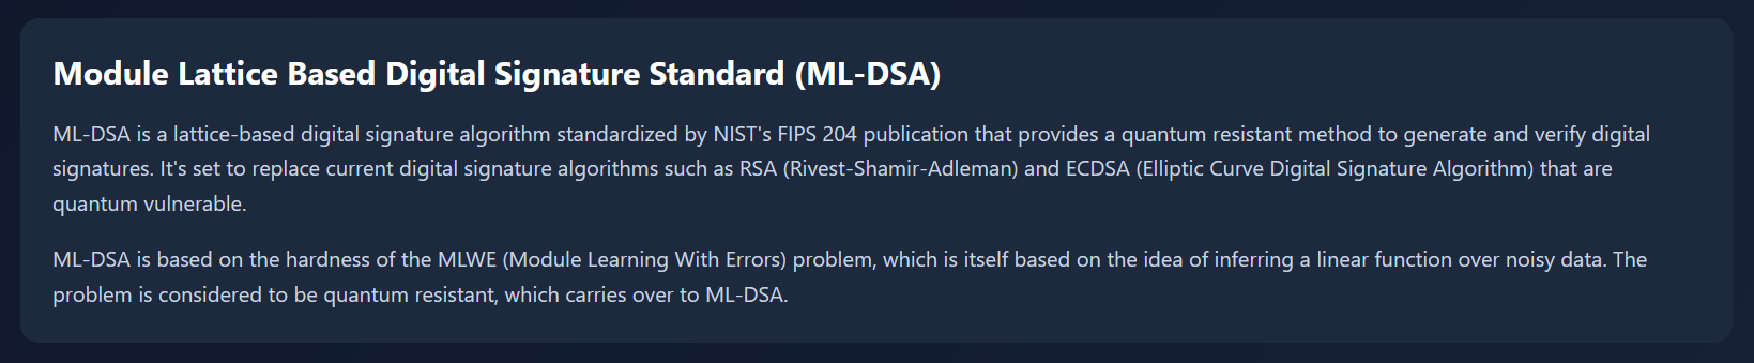
\includegraphics[width=.48\linewidth]{assets/pdfs/about_mldsa.pdf}
\caption{ML-DSA about component}
\label{fig11}
\end{figure}

ML-DSA is described in terms that should be familiar to most people with an awareness of cryptography. Rather than focusing on the underlying lattice mathematics, the description emphasizes practical concepts such as signature generation, signature verification, quantum resistant security, and the relationship between ML-DSA and existing algorithms like RSA and ECDSA. This keeps the introduction accessible while preserving the key ideas needed to understand its role in modern cryptographic systems.

After that is a section that briefly explains each stage of the chosen algorithm and provides an animation showing the scheme in use.

\begin{figure}[H]
\centering
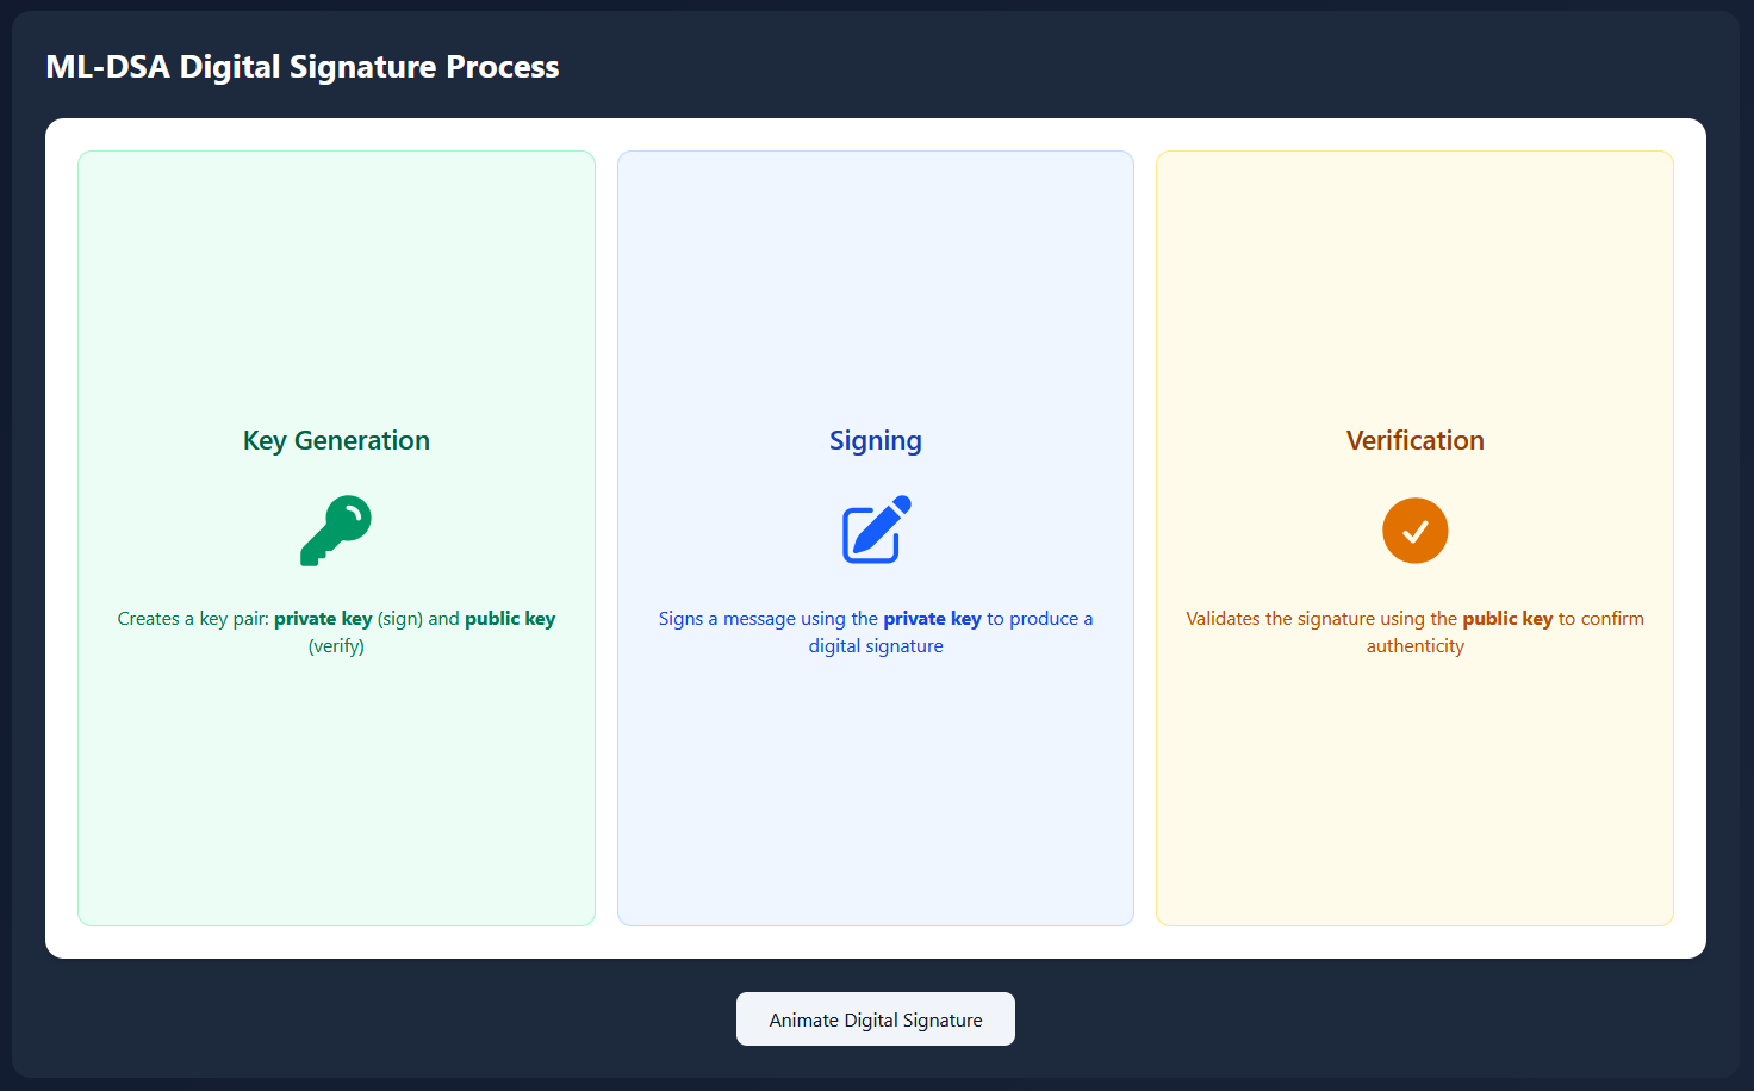
\includegraphics[width=.48\linewidth]{assets/pdfs/process_overview.pdf}
\caption{ML-DSA Process}
\label{fig12}
\end{figure}

The section first shows a short description of the purpose of each stage of either algorithm. For ML-DSA, this is key generation, signing, and verification. If the user clicks the button on the bottom of the section, an animation will play that shows the scheme being used in a simplified abstraction of a real world example.

\begin{figure}[H]
\centering
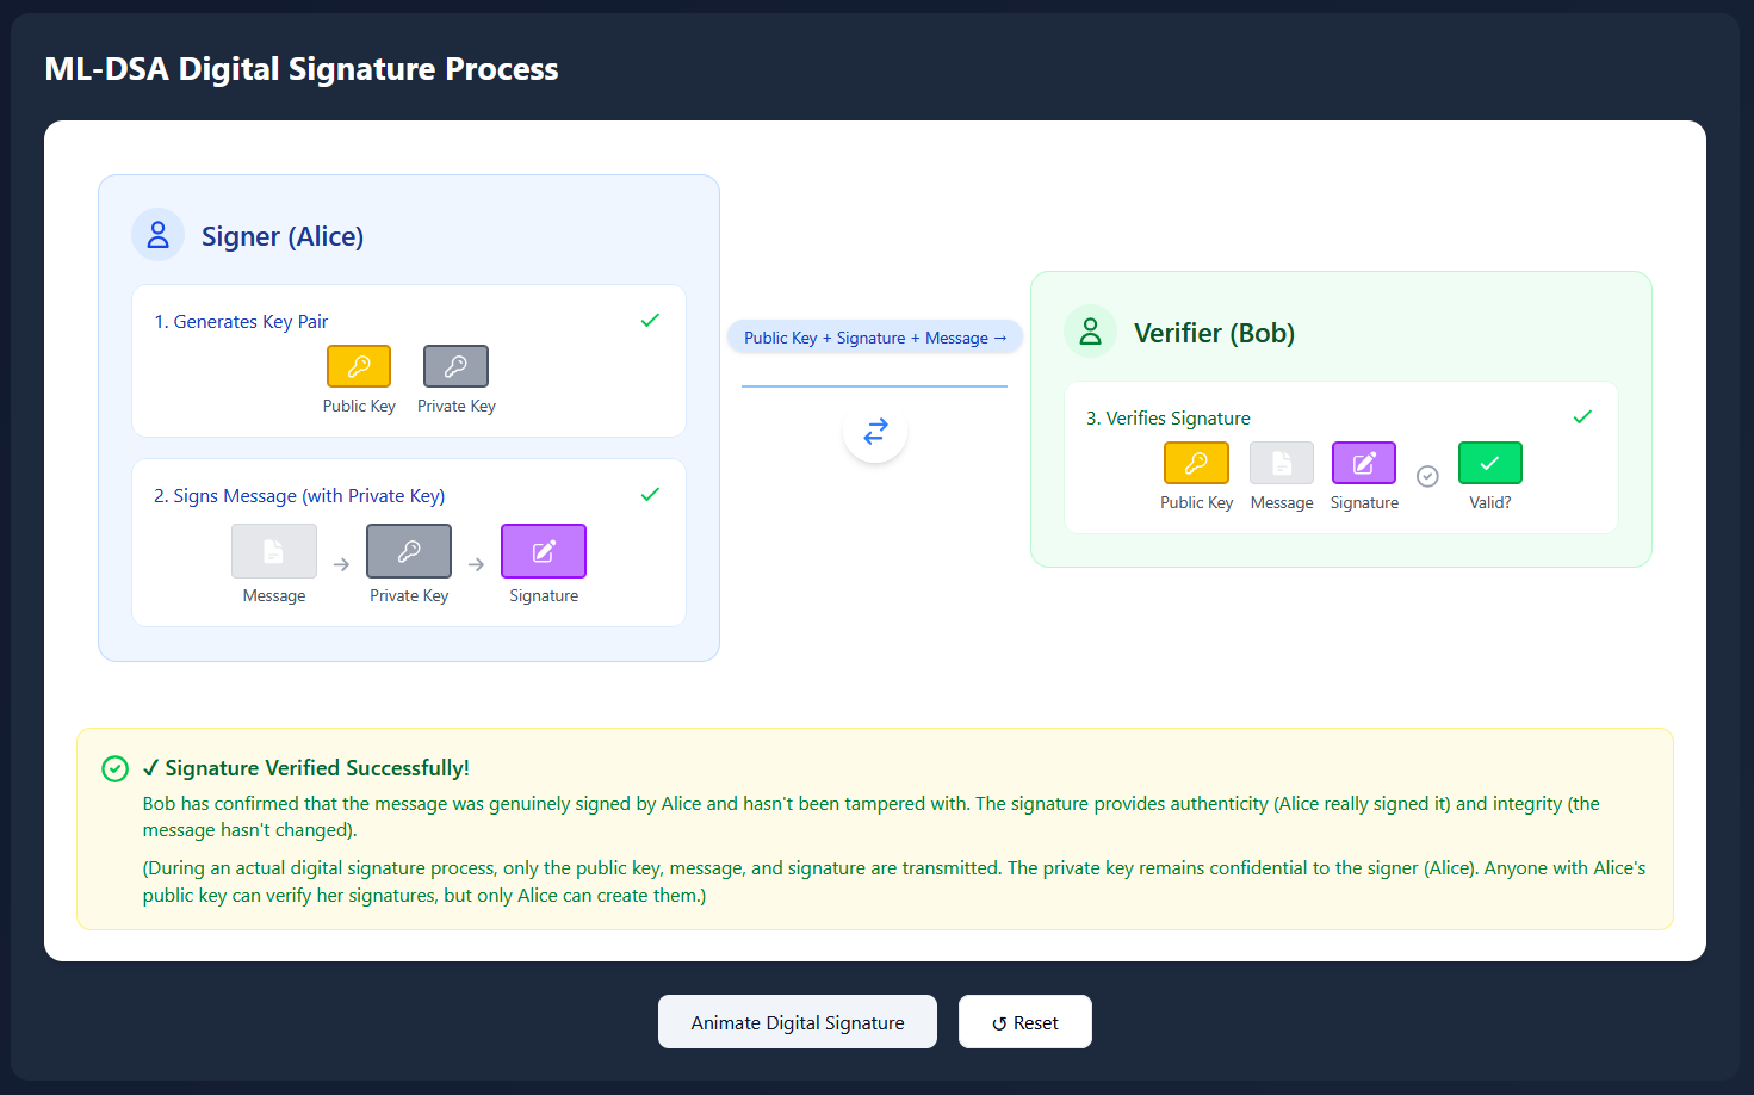
\includegraphics[width=.48\linewidth]{assets/pdfs/process_animation.pdf}
\caption{ML-DSA Process Animation}
\label{fig13}
\end{figure}

Below that is a section that displays an instance of the algorithm in full, including the variables and functions involved in its inner workings. Within it are four different components that each have different functions.

\begin{figure}[H]
\centering
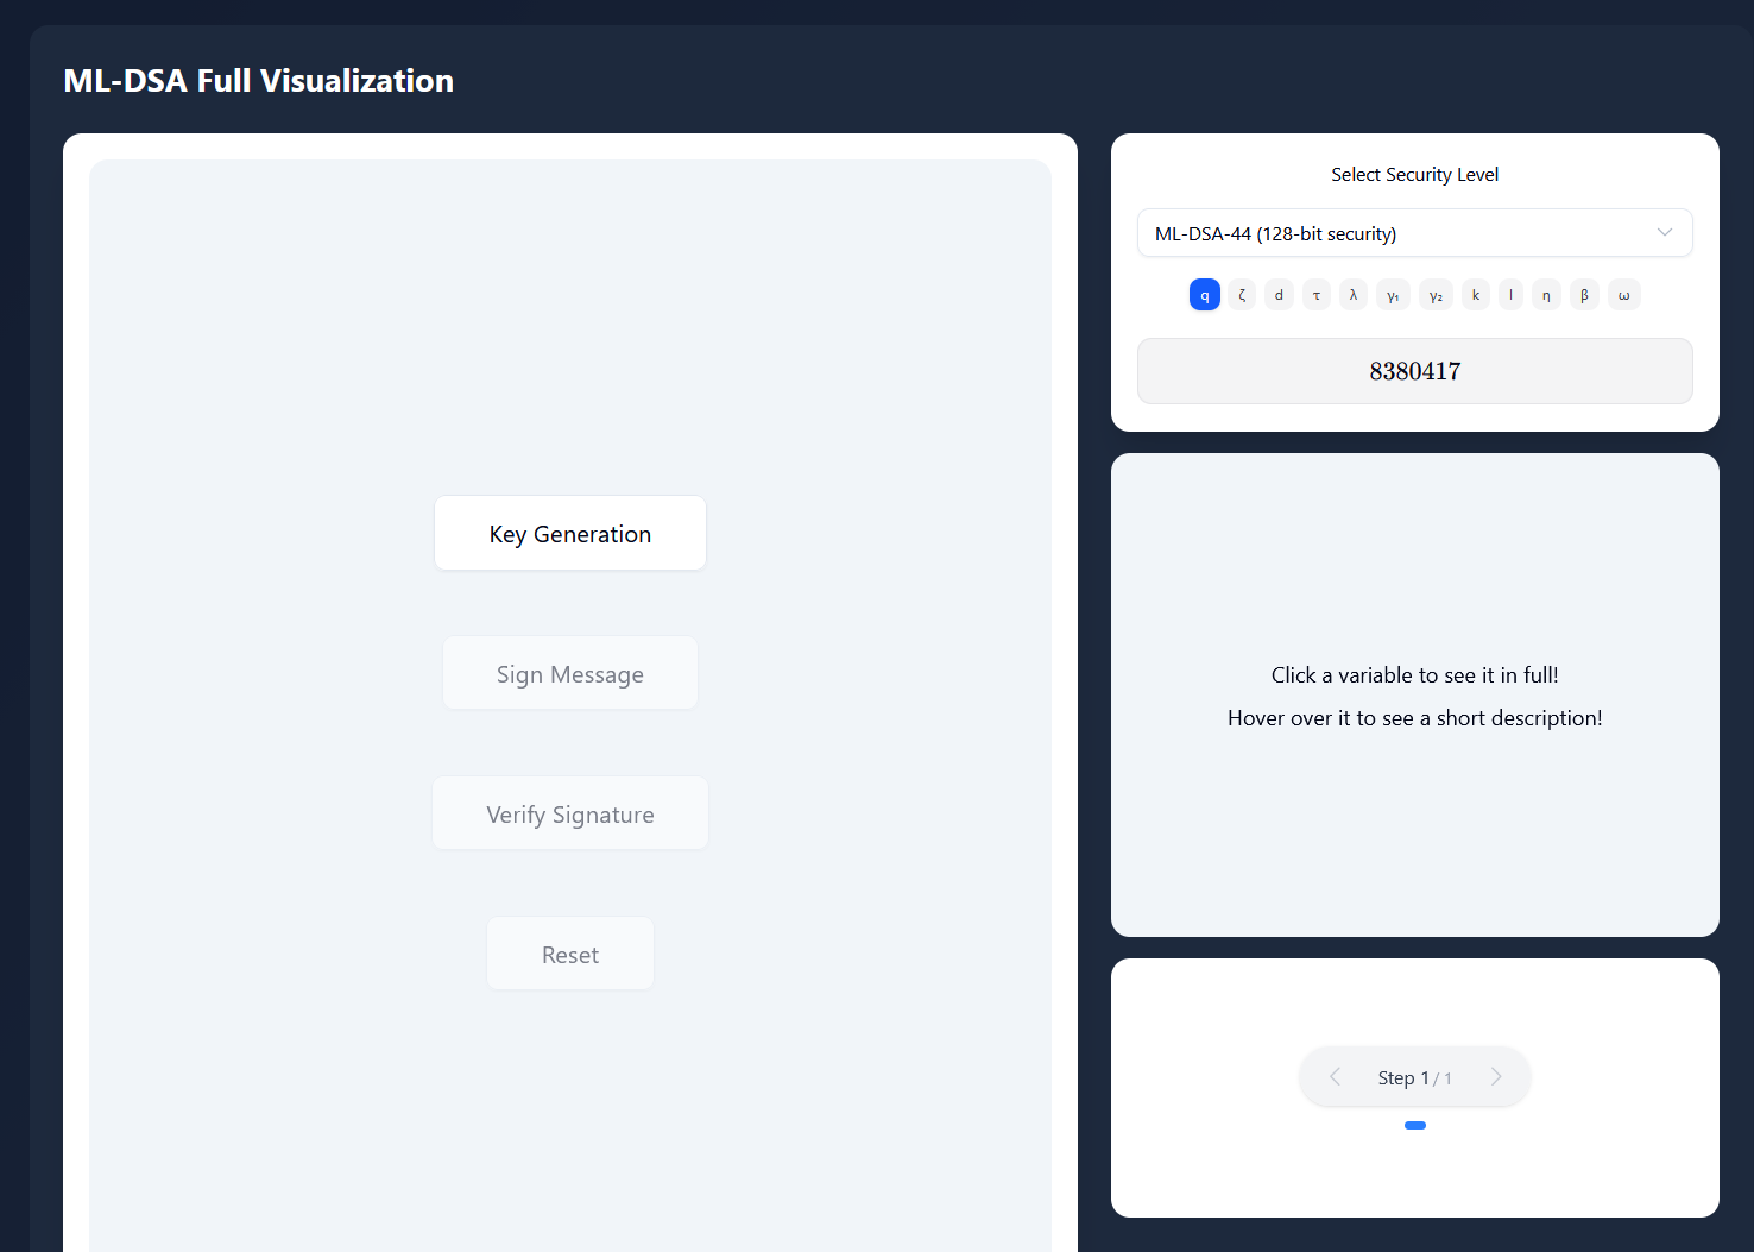
\includegraphics[width=.48\linewidth]{assets/pdfs/mldsa_fullvisualization.pdf}
\caption{ML-DSA Full Animation Section}
\label{fig14}
\end{figure}

Starting from the top-right is the security level selection component. The user can pick between the available security levels, though it defaults to the lowest security level. Beneath the selection, the parameters of the chosen security level are displayed. Whenever a security level is chosen, the visualization is reset and a new instance of ML-DSA is created according to the new security level.

\begin{figure}[H]
\centering
\begin{subfigure}{.5\textwidth}
  \centering
  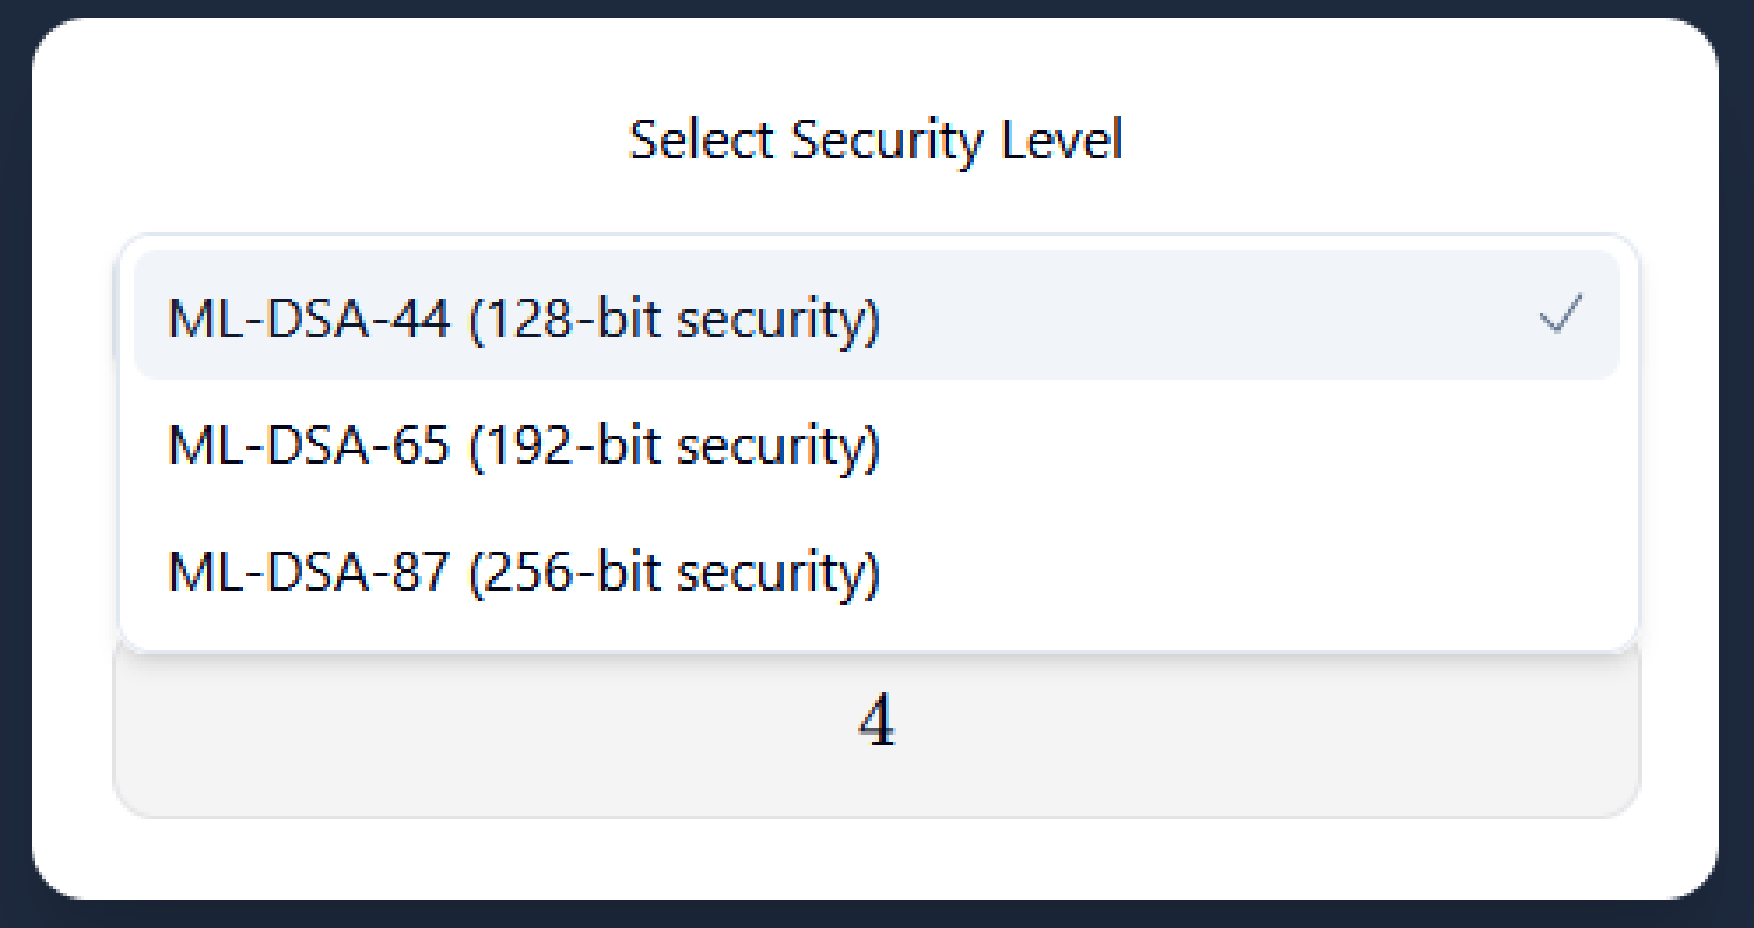
\includegraphics[width=.4\linewidth]{assets/pdfs/selectsecurity.pdf}
  \caption{Security level selection}
  \label{fig:sub8}
\end{subfigure}%
\begin{subfigure}{.5\textwidth}
  \centering
  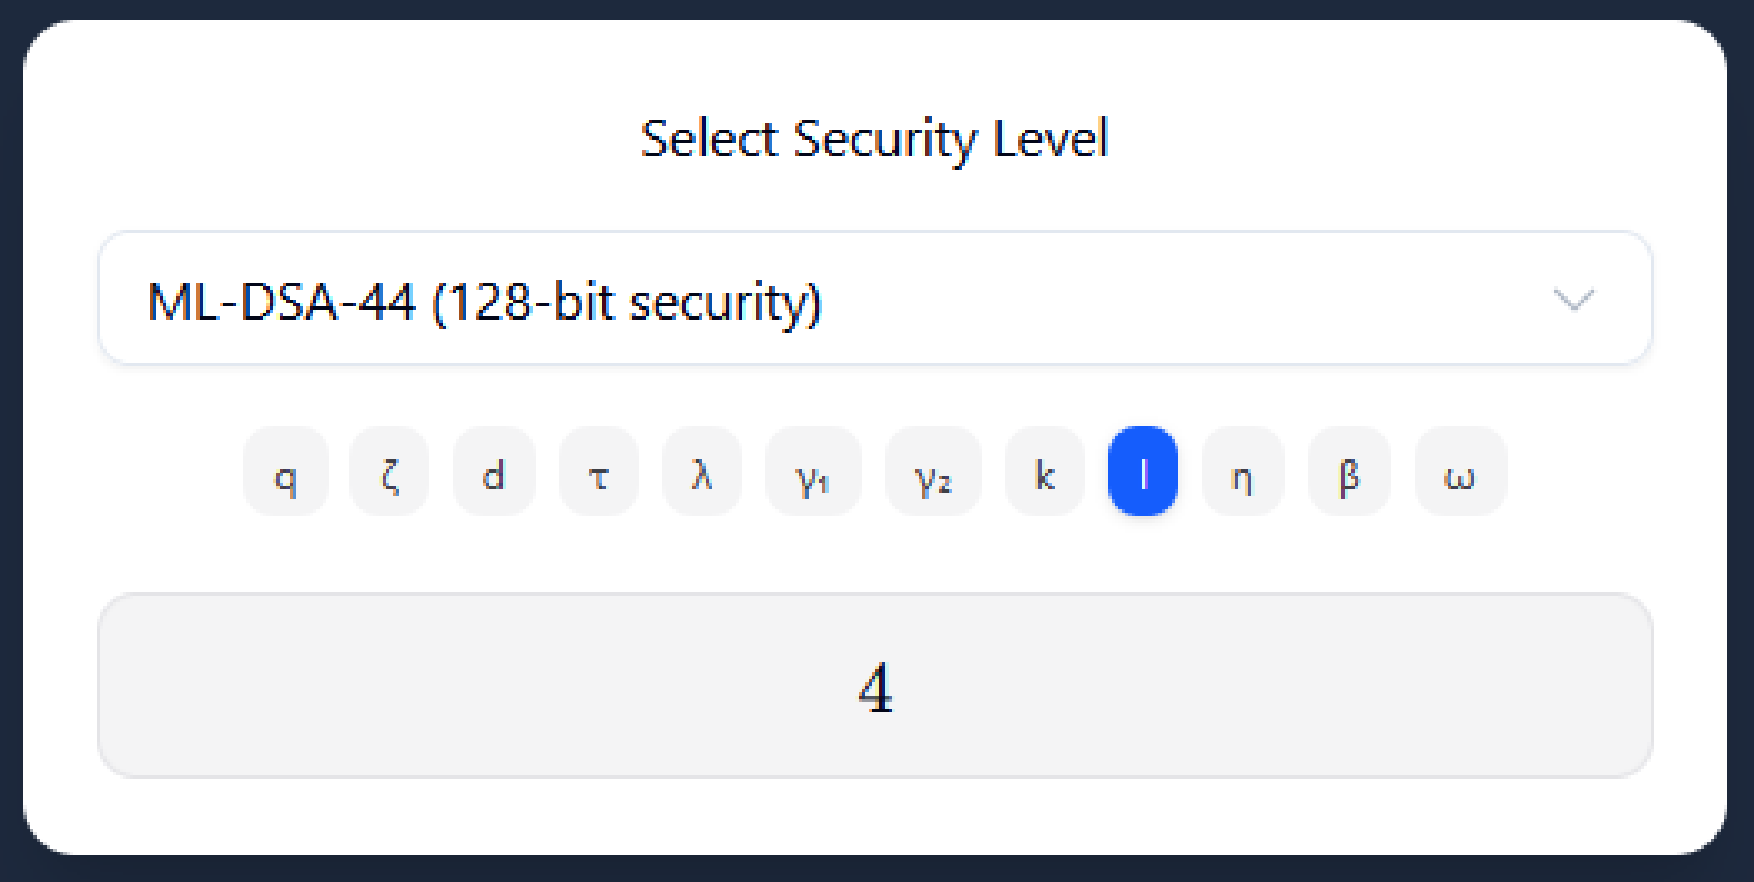
\includegraphics[width=.4\linewidth]{assets/pdfs/parameters.pdf}
  \caption{Parameters per security level}
  \label{fig:sub9}
\end{subfigure}
\caption{Security Level Selection Component}
\label{fig:seclevel}
\end{figure}

The leftmost component is the main part of this section. It contains four buttons. The first three lead to visualizations of the three stages of ML-DSA. The visualizations come in the form of step-by-step abstractions of the main algorithms of each stage, complete with explanations on the relevant variables and functions.
In ML-DSA specifically, there is an input section for the signing stage that only appears after the key generation stage has been gone through. It needs to be filled in before the signing stage can be accessed, and it is the only actual input from the user that can be used for running an instance of ML-DSA aside from security level selection.

\begin{figure}[H]
\centering
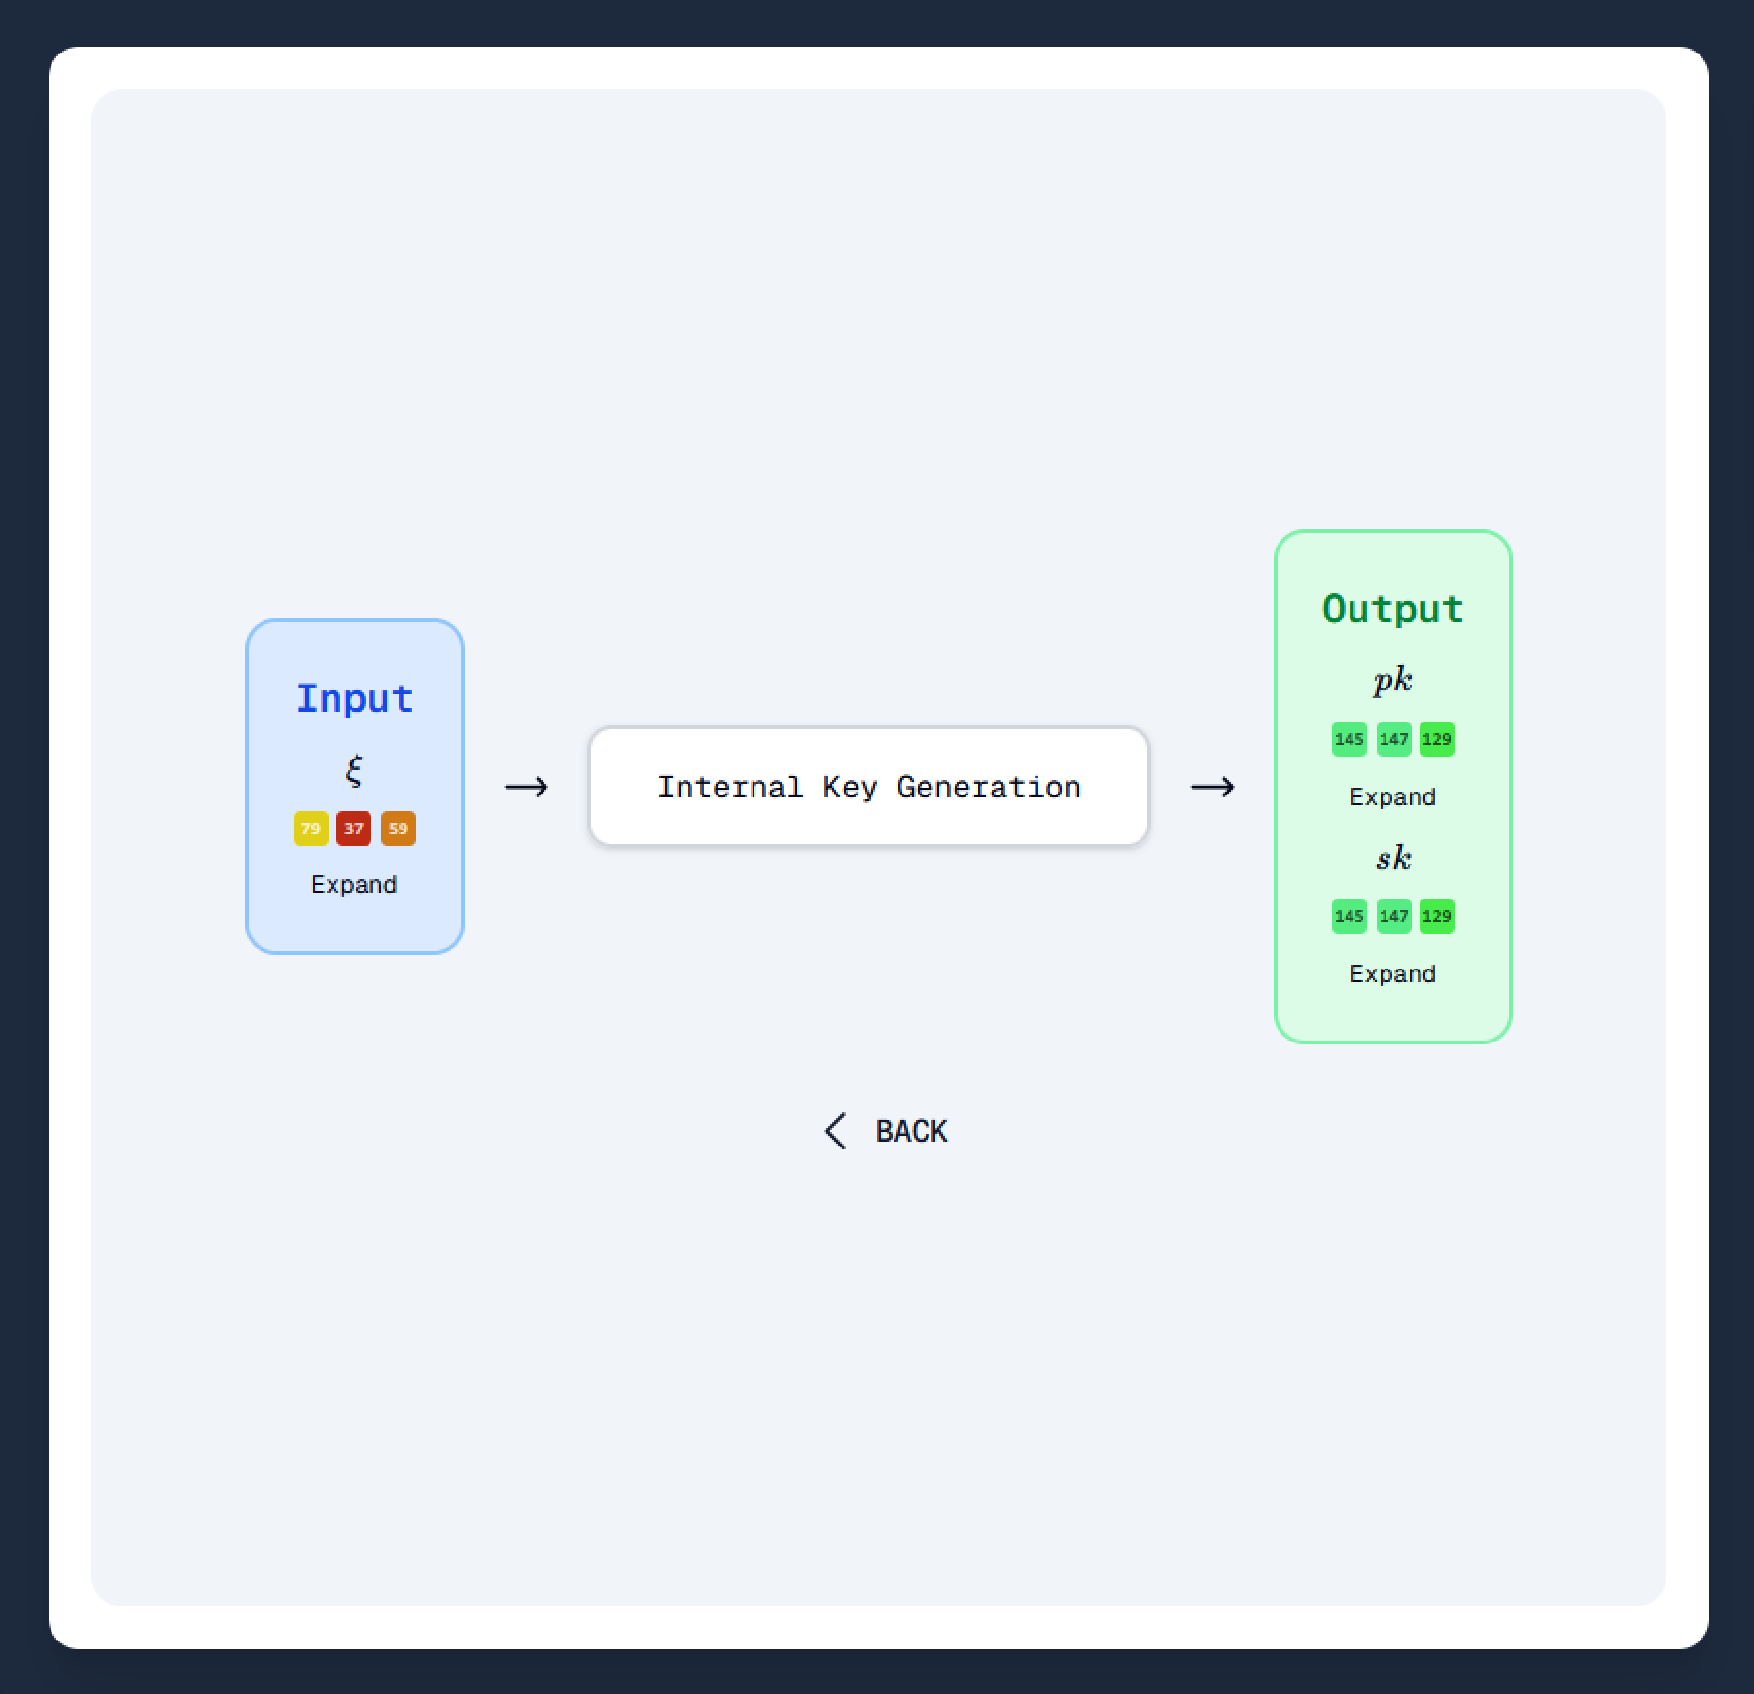
\includegraphics[width=.48\linewidth]{assets/pdfs/leftmost_component.pdf}
\caption{ML-DSA Full Animation Section}
\label{fig15}
\end{figure}

\begin{figure}[H]
\centering
\begin{subfigure}{.5\textwidth}
  \centering
  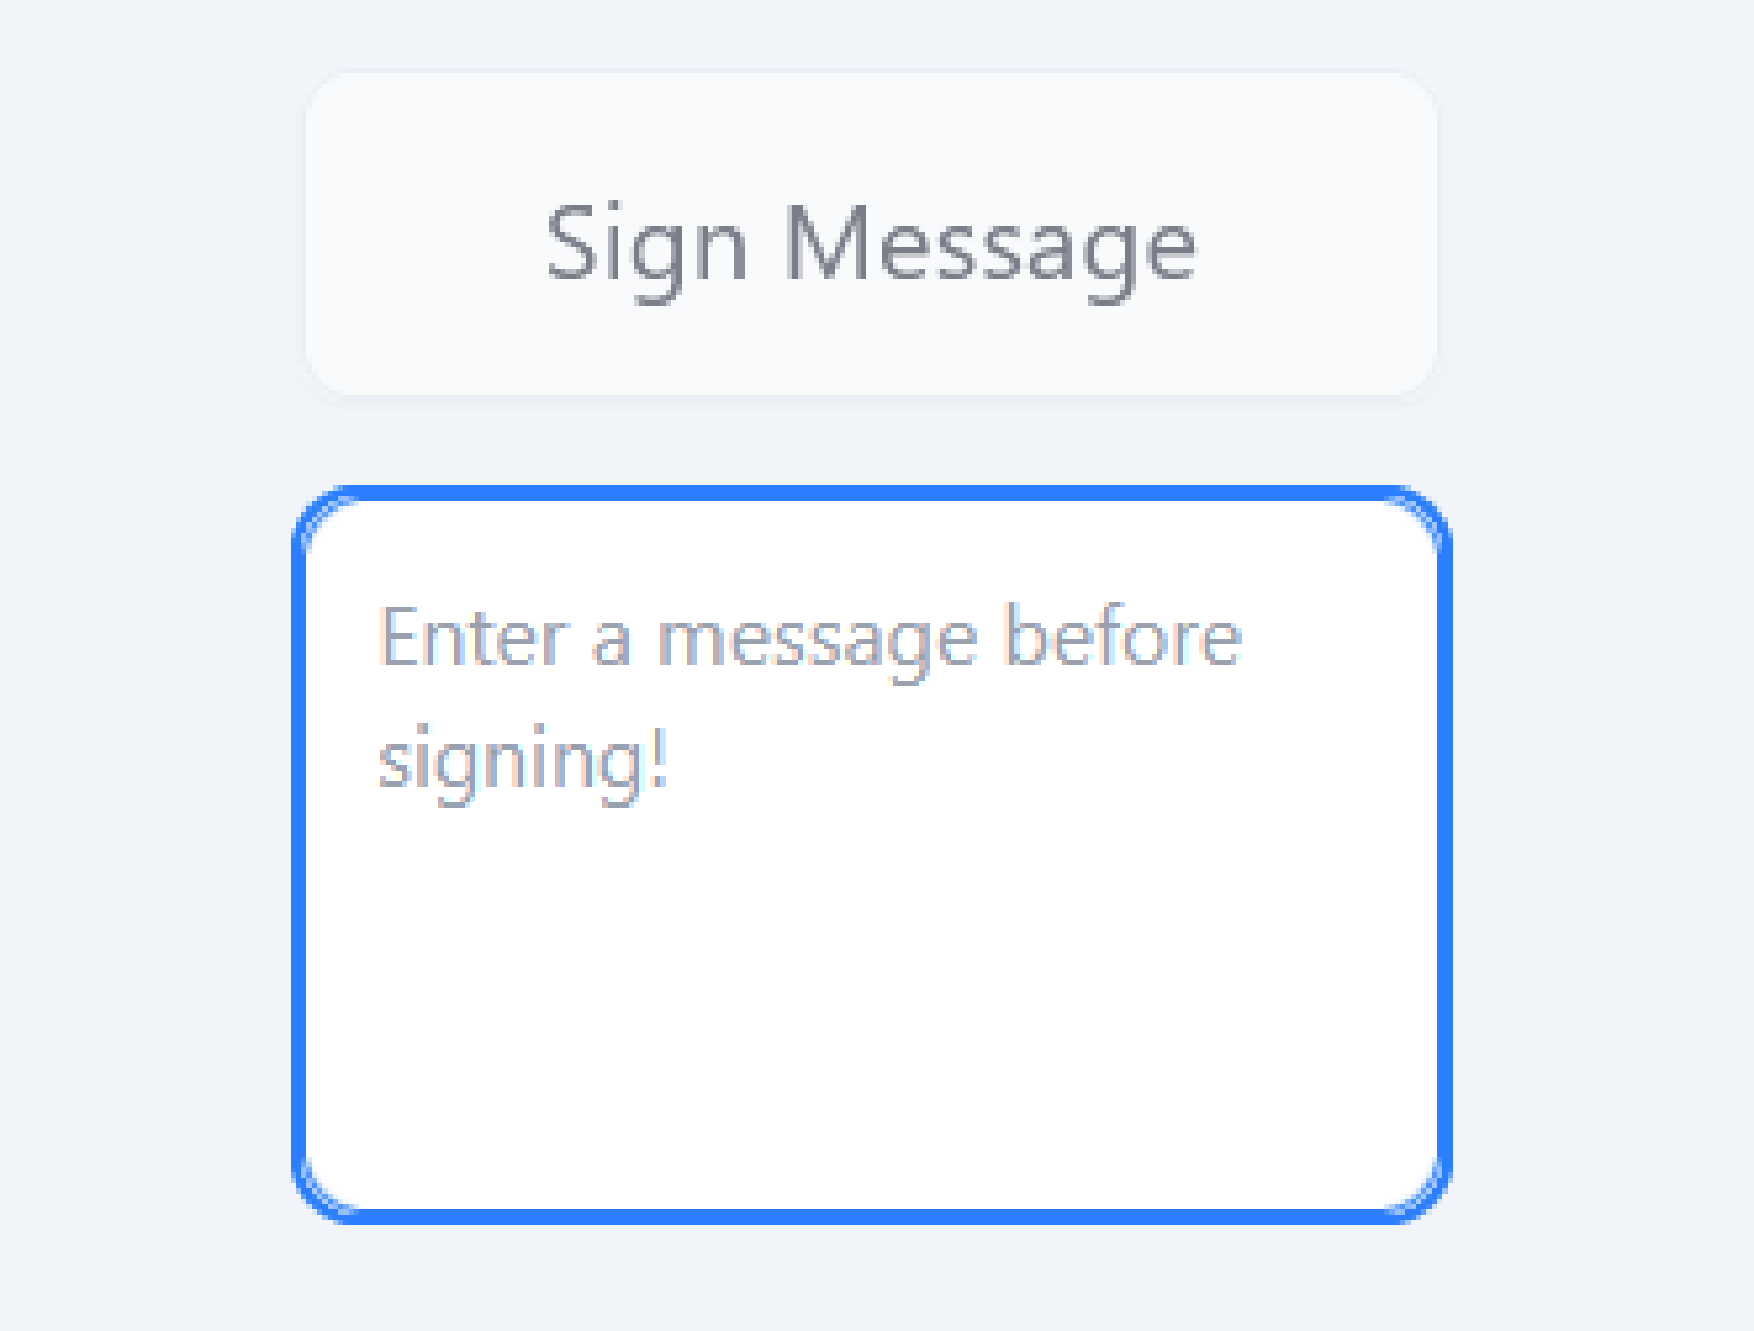
\includegraphics[width=.4\linewidth]{assets/pdfs/sign_input1.pdf}
  \caption{Empty message input}
  \label{fig:sub6}
\end{subfigure}%
\begin{subfigure}{.5\textwidth}
  \centering
  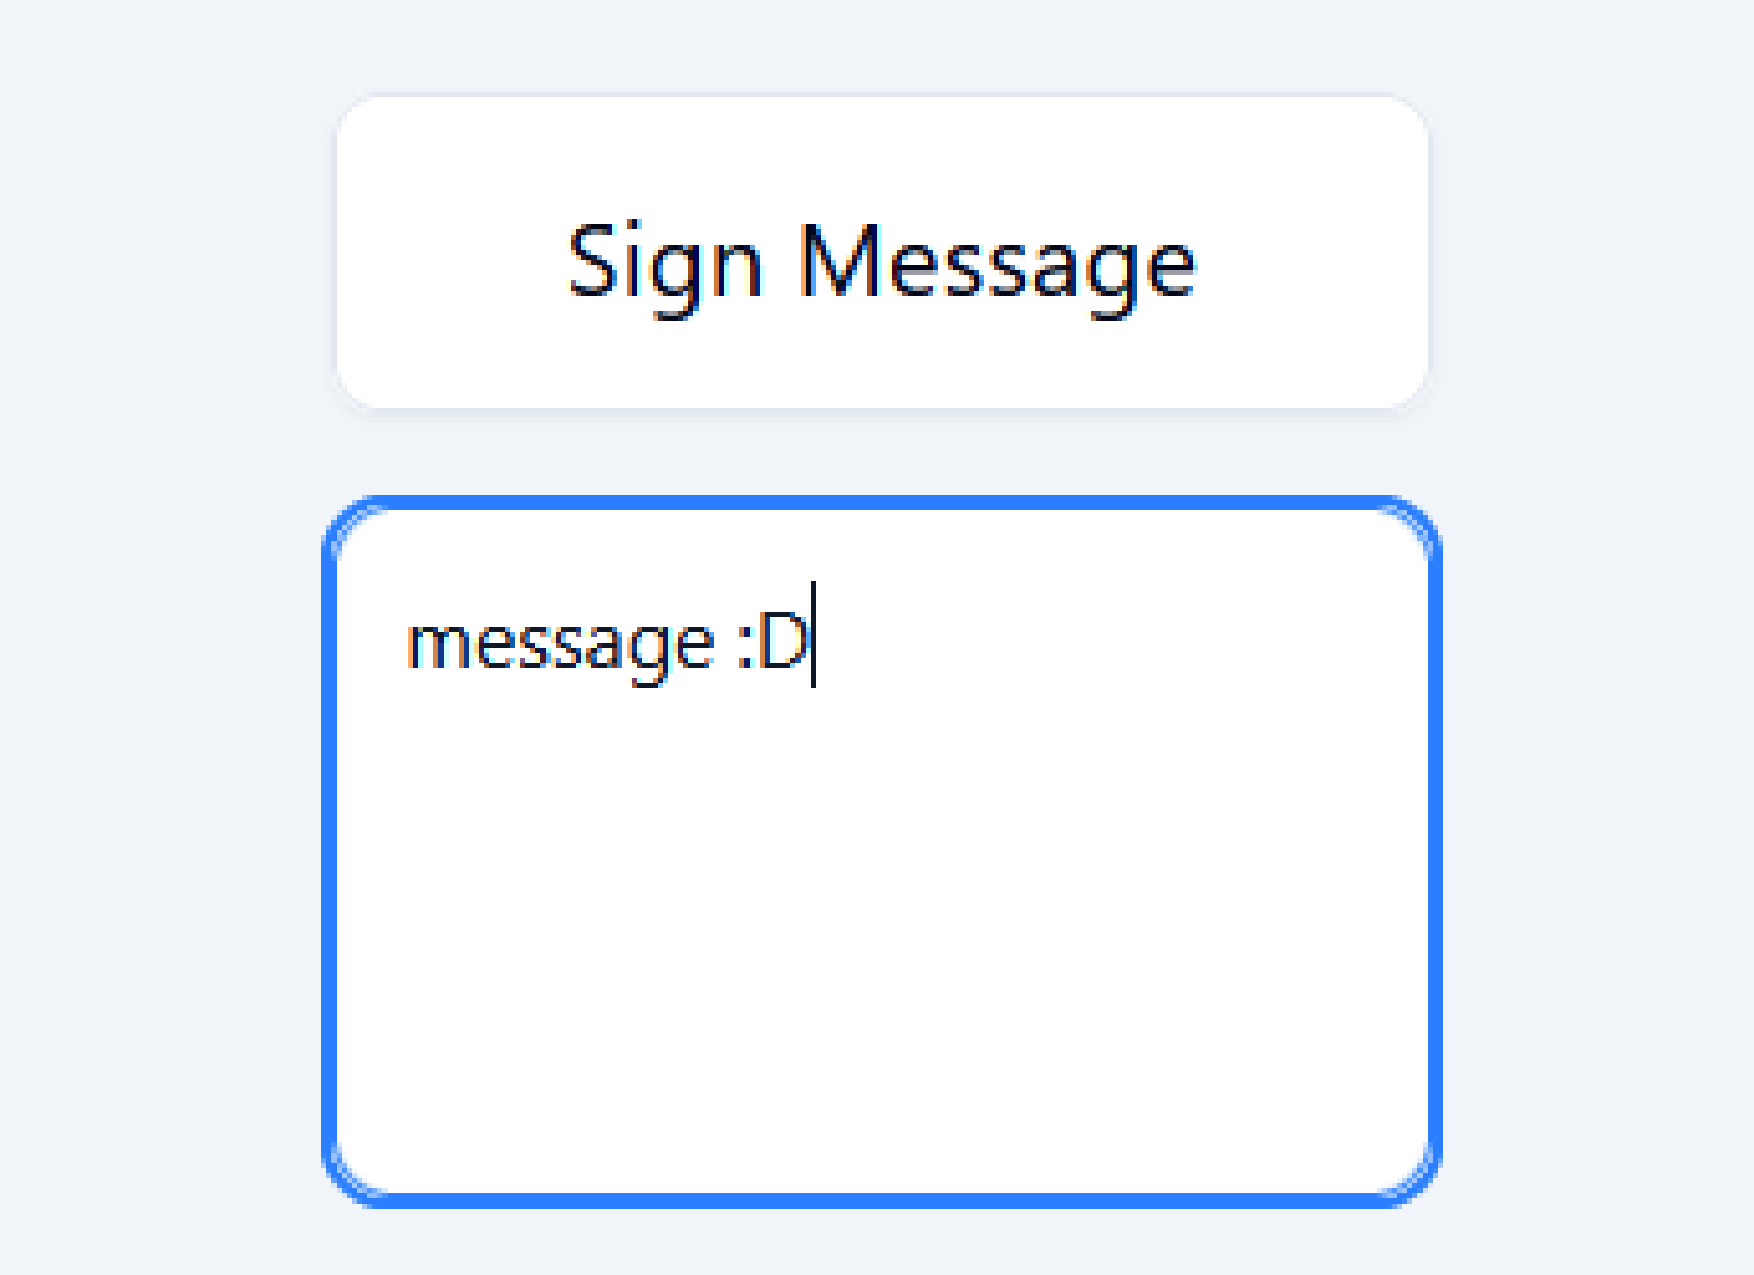
\includegraphics[width=.4\linewidth]{assets/pdfs/sign_input2.pdf}
  \caption{Filled message input}
  \label{fig:sub7}
\end{subfigure}
\caption{Input for Sign Message}
\label{fig:signmessage}
\end{figure}

As interactivity forces engagement and engagement leads to more effective learning \cite{HUNDHAUSEN2002259}, these visualizations are interactive. Each variable is displayed in the form of a colored matrix which can be expanded on click to show more values. The values represent the coefficients of the polynomials that make up the variables. When the matrix is hovered on, a popup will appear beside it that describes what it is and provides extra details relating to what it is used for or how it is calculated.

\begin{figure}[H]
\centering
\begin{subfigure}{.3\textwidth}
  \centering
  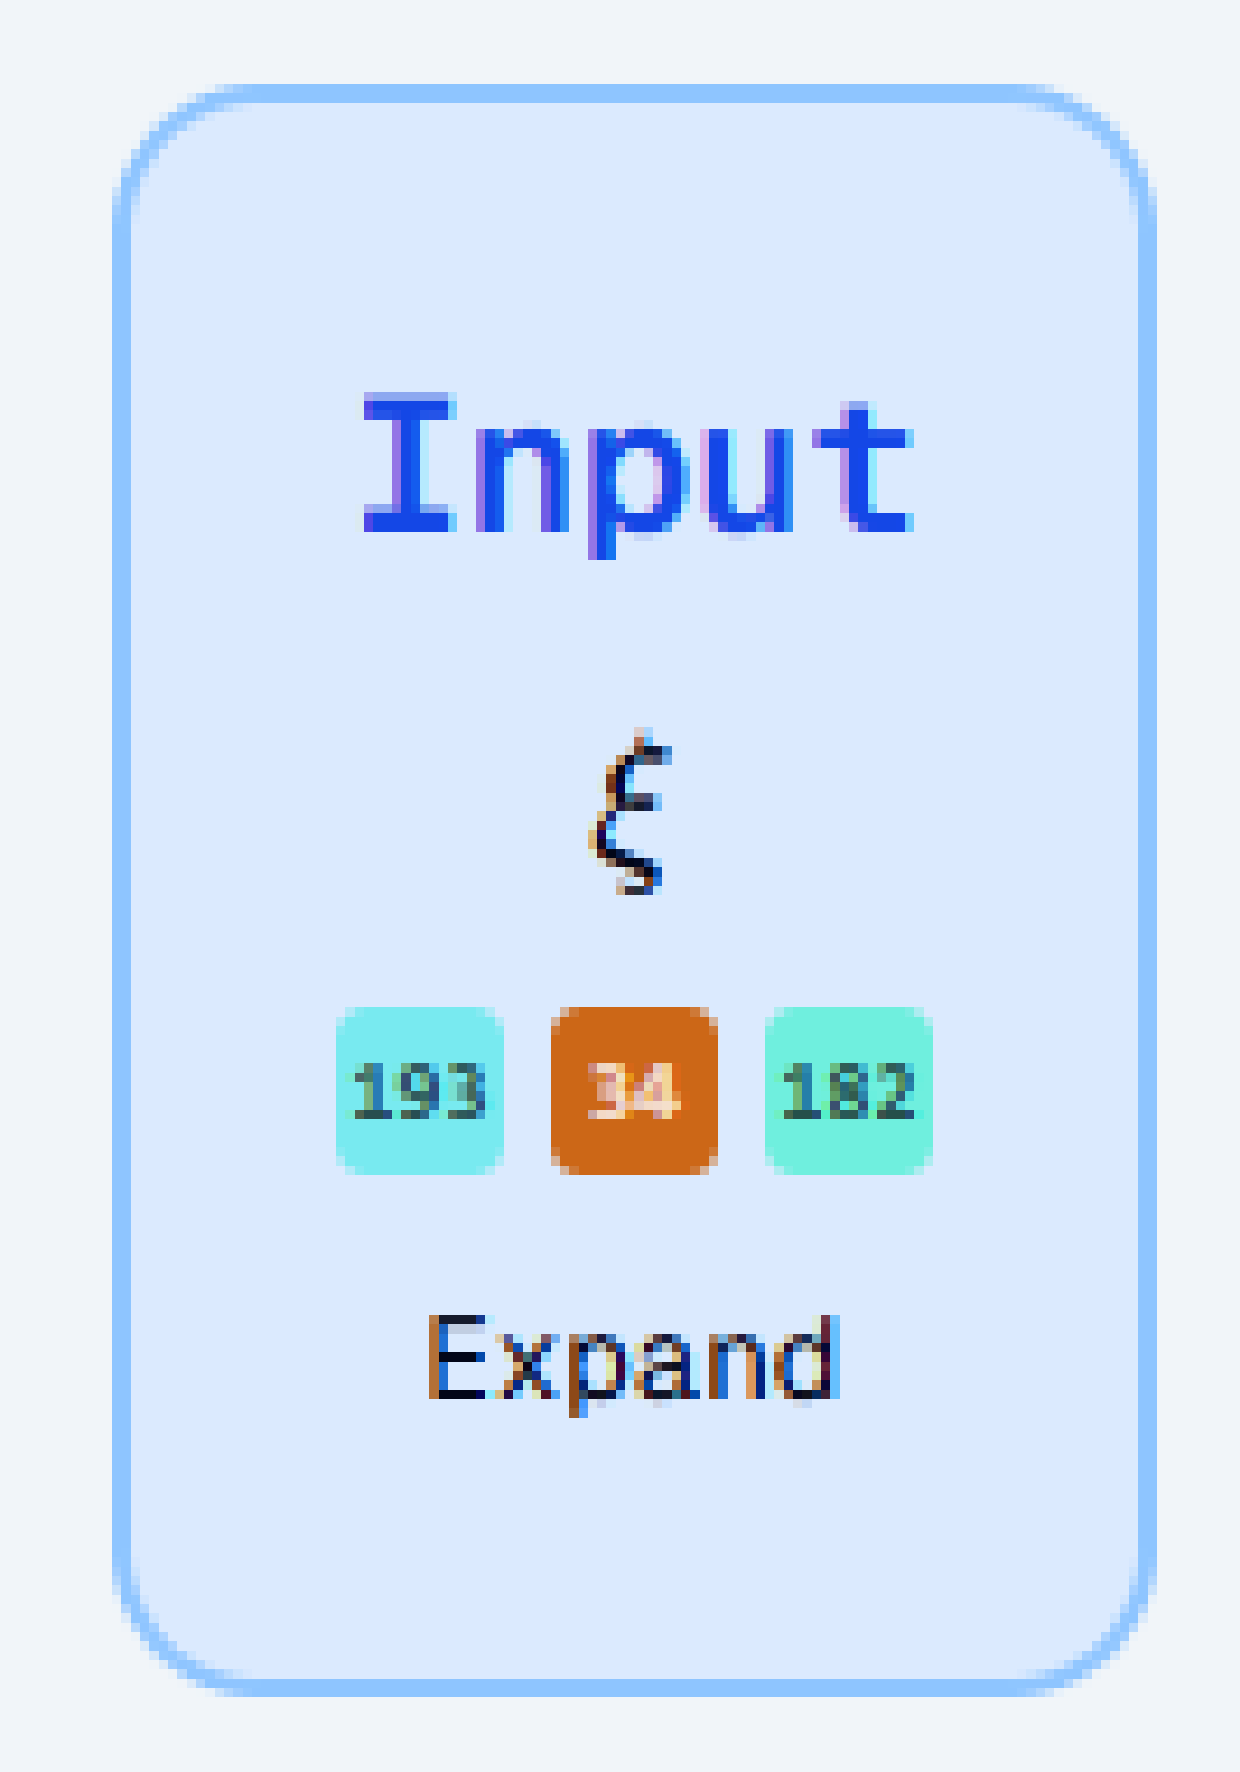
\includegraphics[width=.3\linewidth]{assets/pdfs/unexpanded.pdf}
  \caption{Unexpanded variable}
  \label{fig:sub1}
\end{subfigure}%
\begin{subfigure}{.3\textwidth}
  \centering
  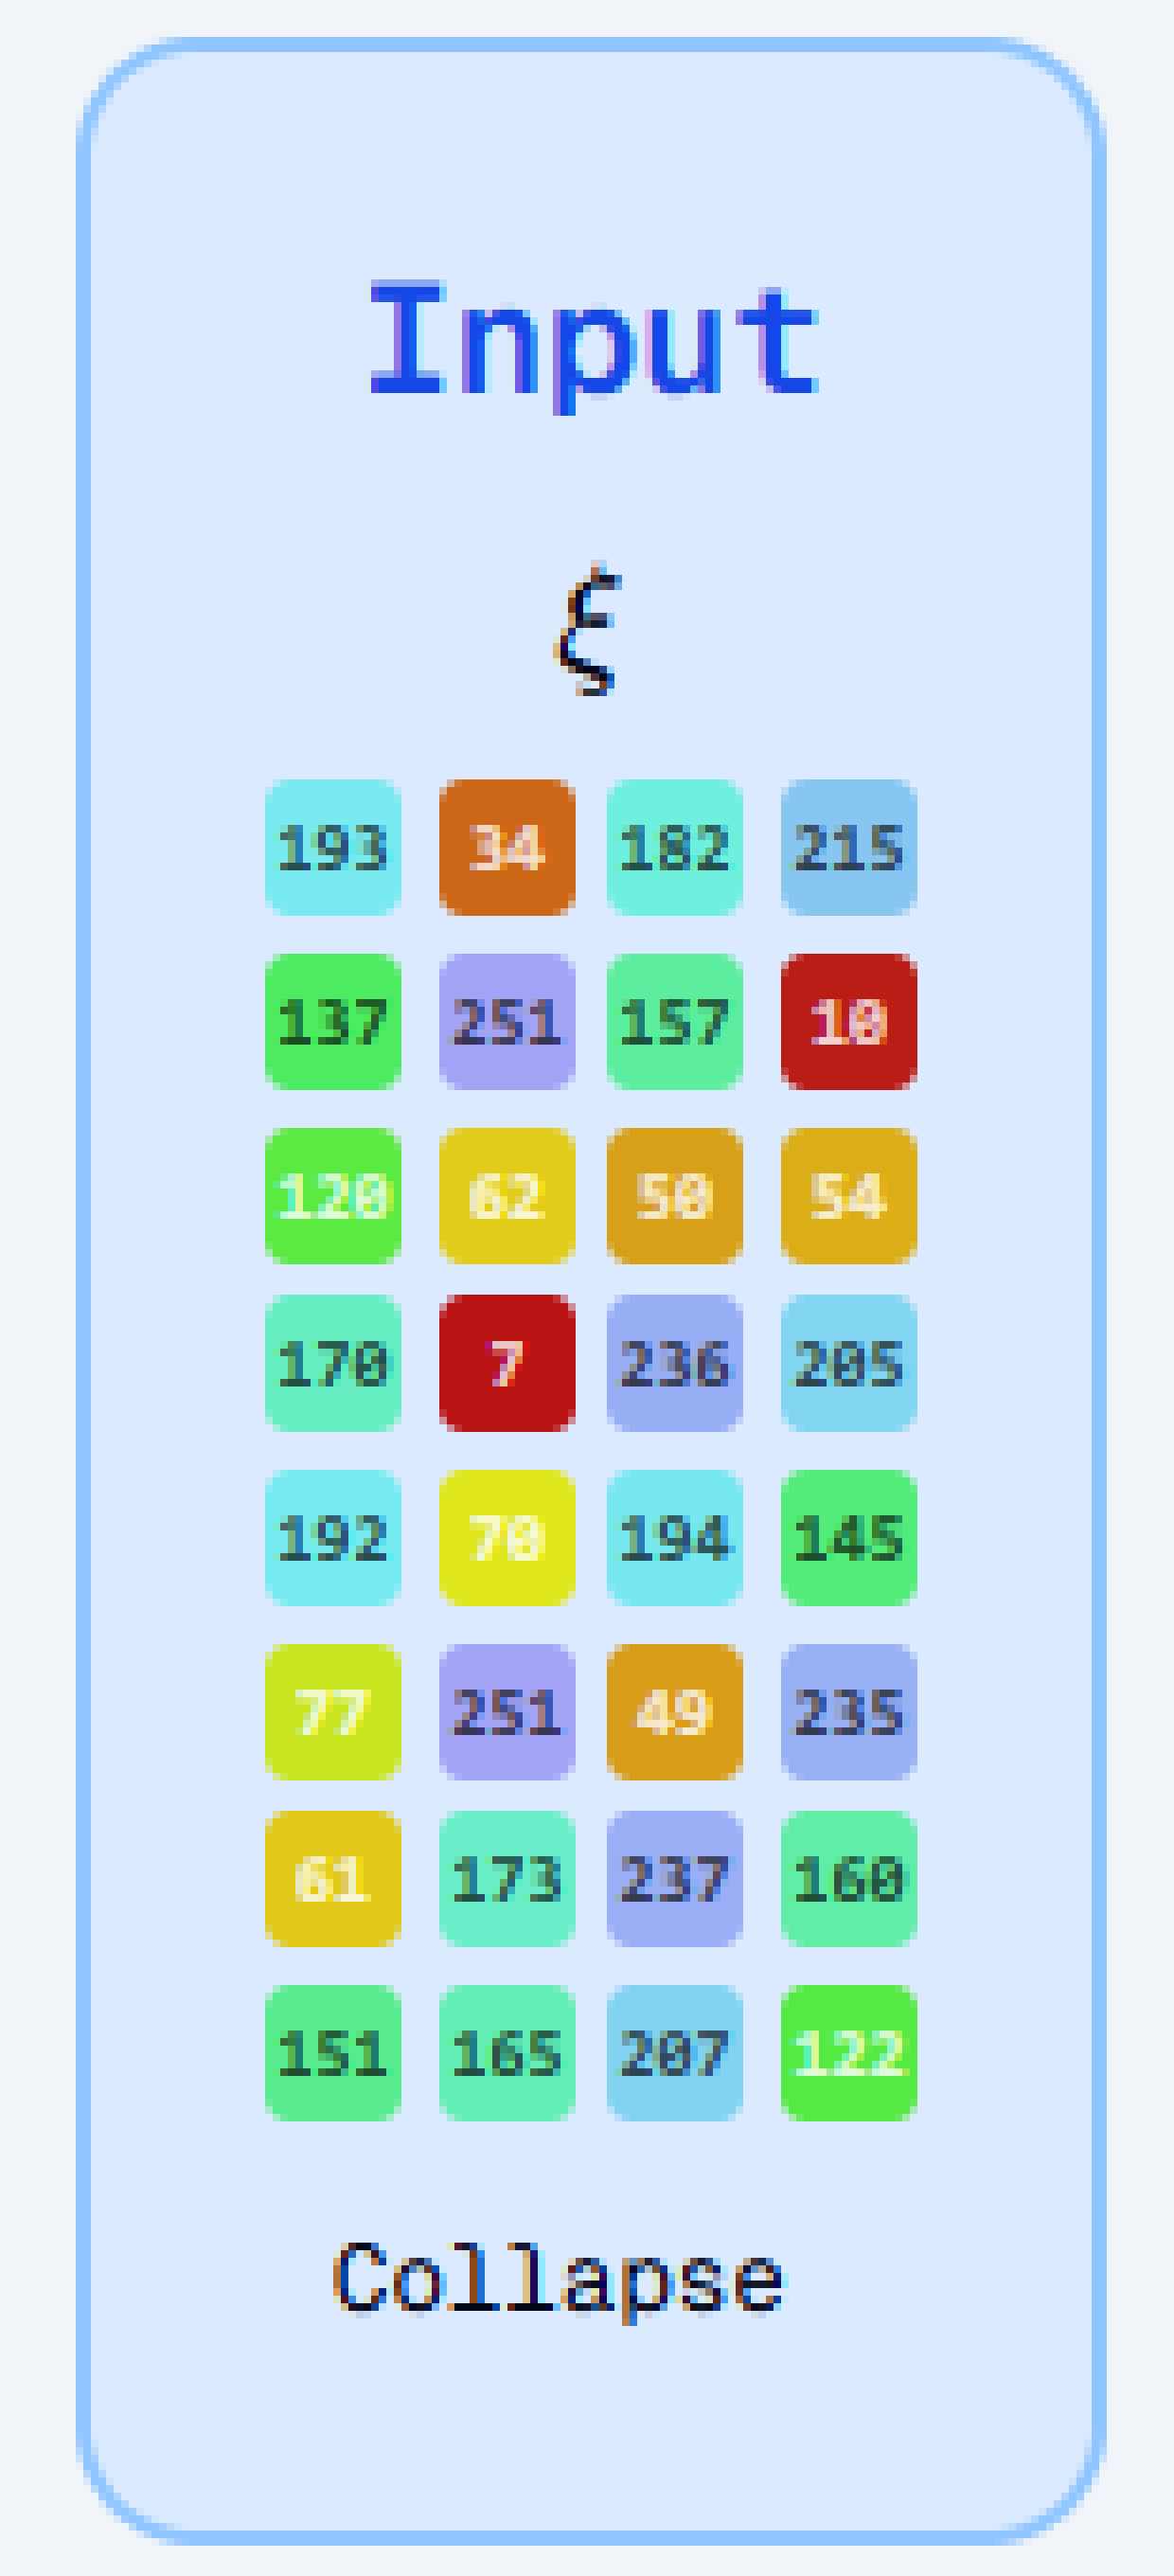
\includegraphics[width=.3\linewidth]{assets/pdfs/expanded.pdf}
  \caption{Expanded variable}
  \label{fig:sub2}
\end{subfigure}
\begin{subfigure}{.3\textwidth}
  \centering
  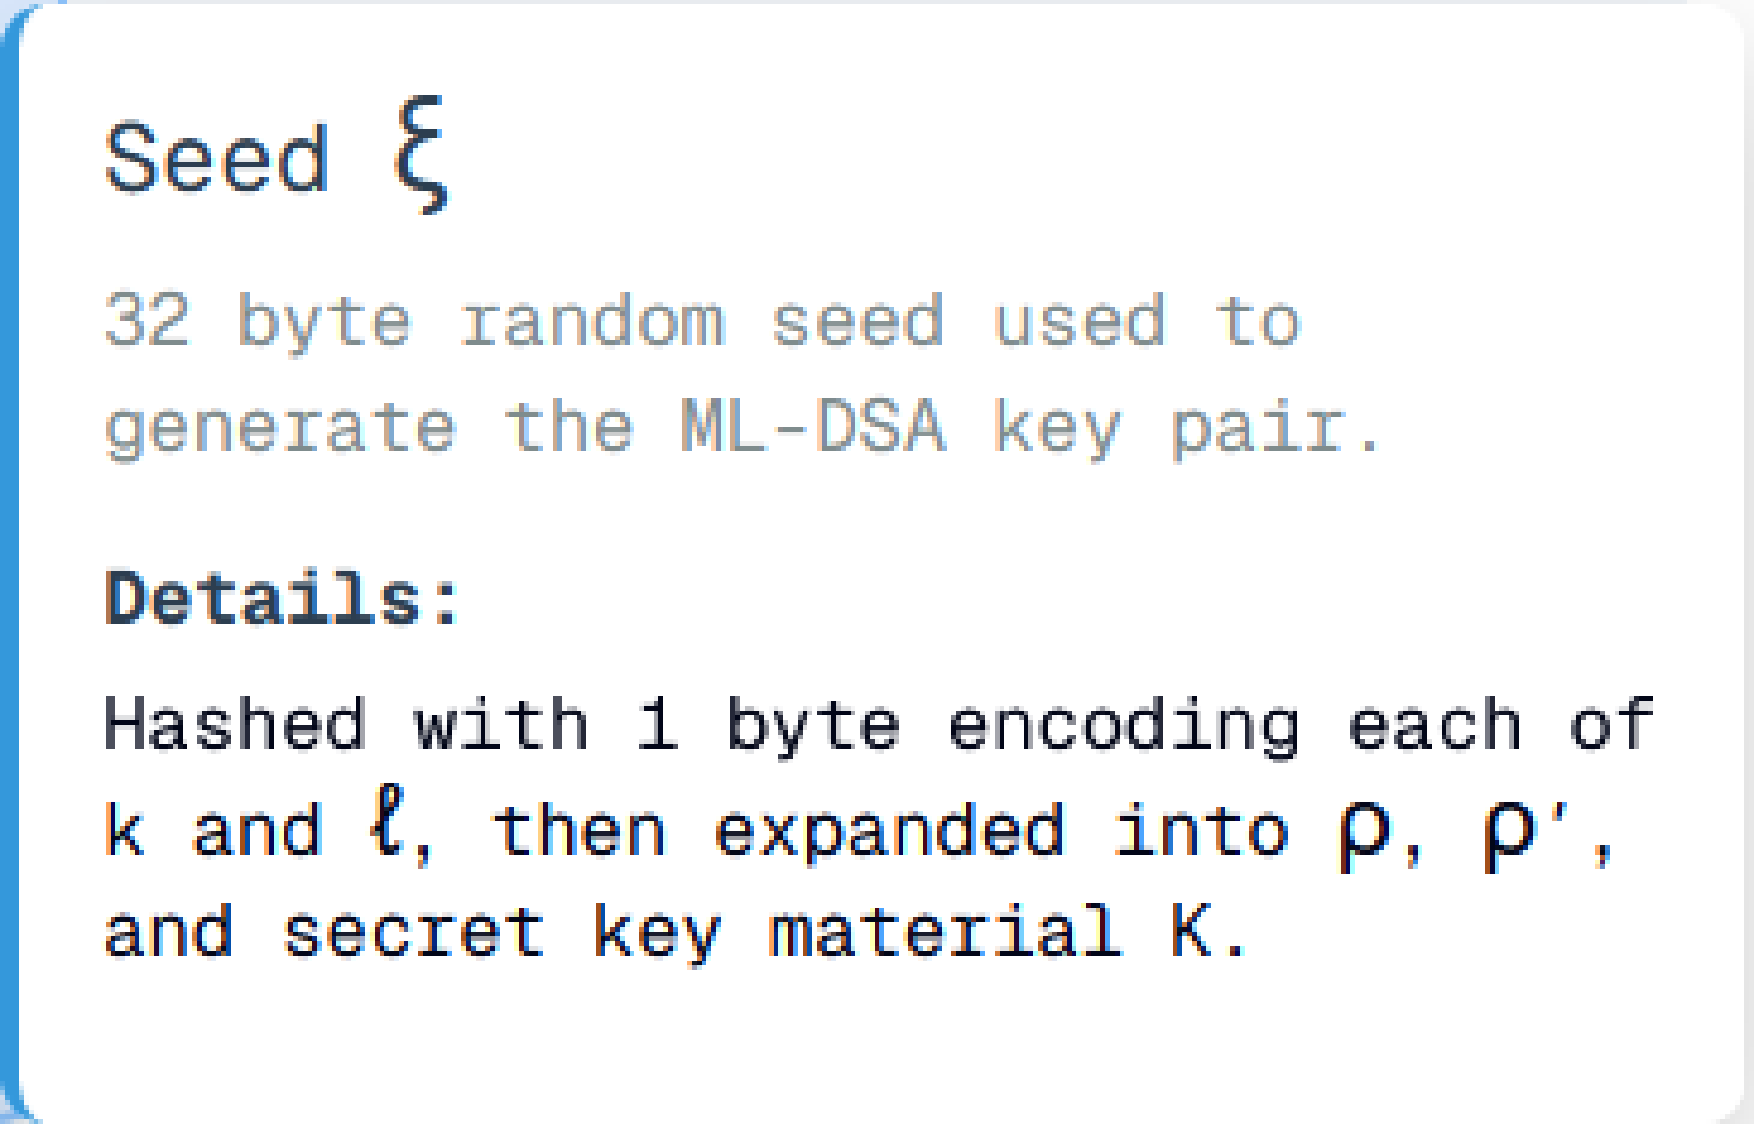
\includegraphics[width=.3\linewidth]{assets/pdfs/popup.pdf}
  \caption{Popup description}
  \label{fig:sub3}
\end{subfigure}
\caption{Variables in the form of colored matrices}
\label{fig:variable}
\end{figure}

Additionally, when a variable is clicked, the component in the middle of the right column will show that variable in scrollable form. This allows for the entire variable to be visible instead of only the first 32 values. There is also an option for the variable to be visible in array form for easier viewing of the values.

\begin{figure}[H]
\centering
\begin{subfigure}{.5\textwidth}
  \centering
  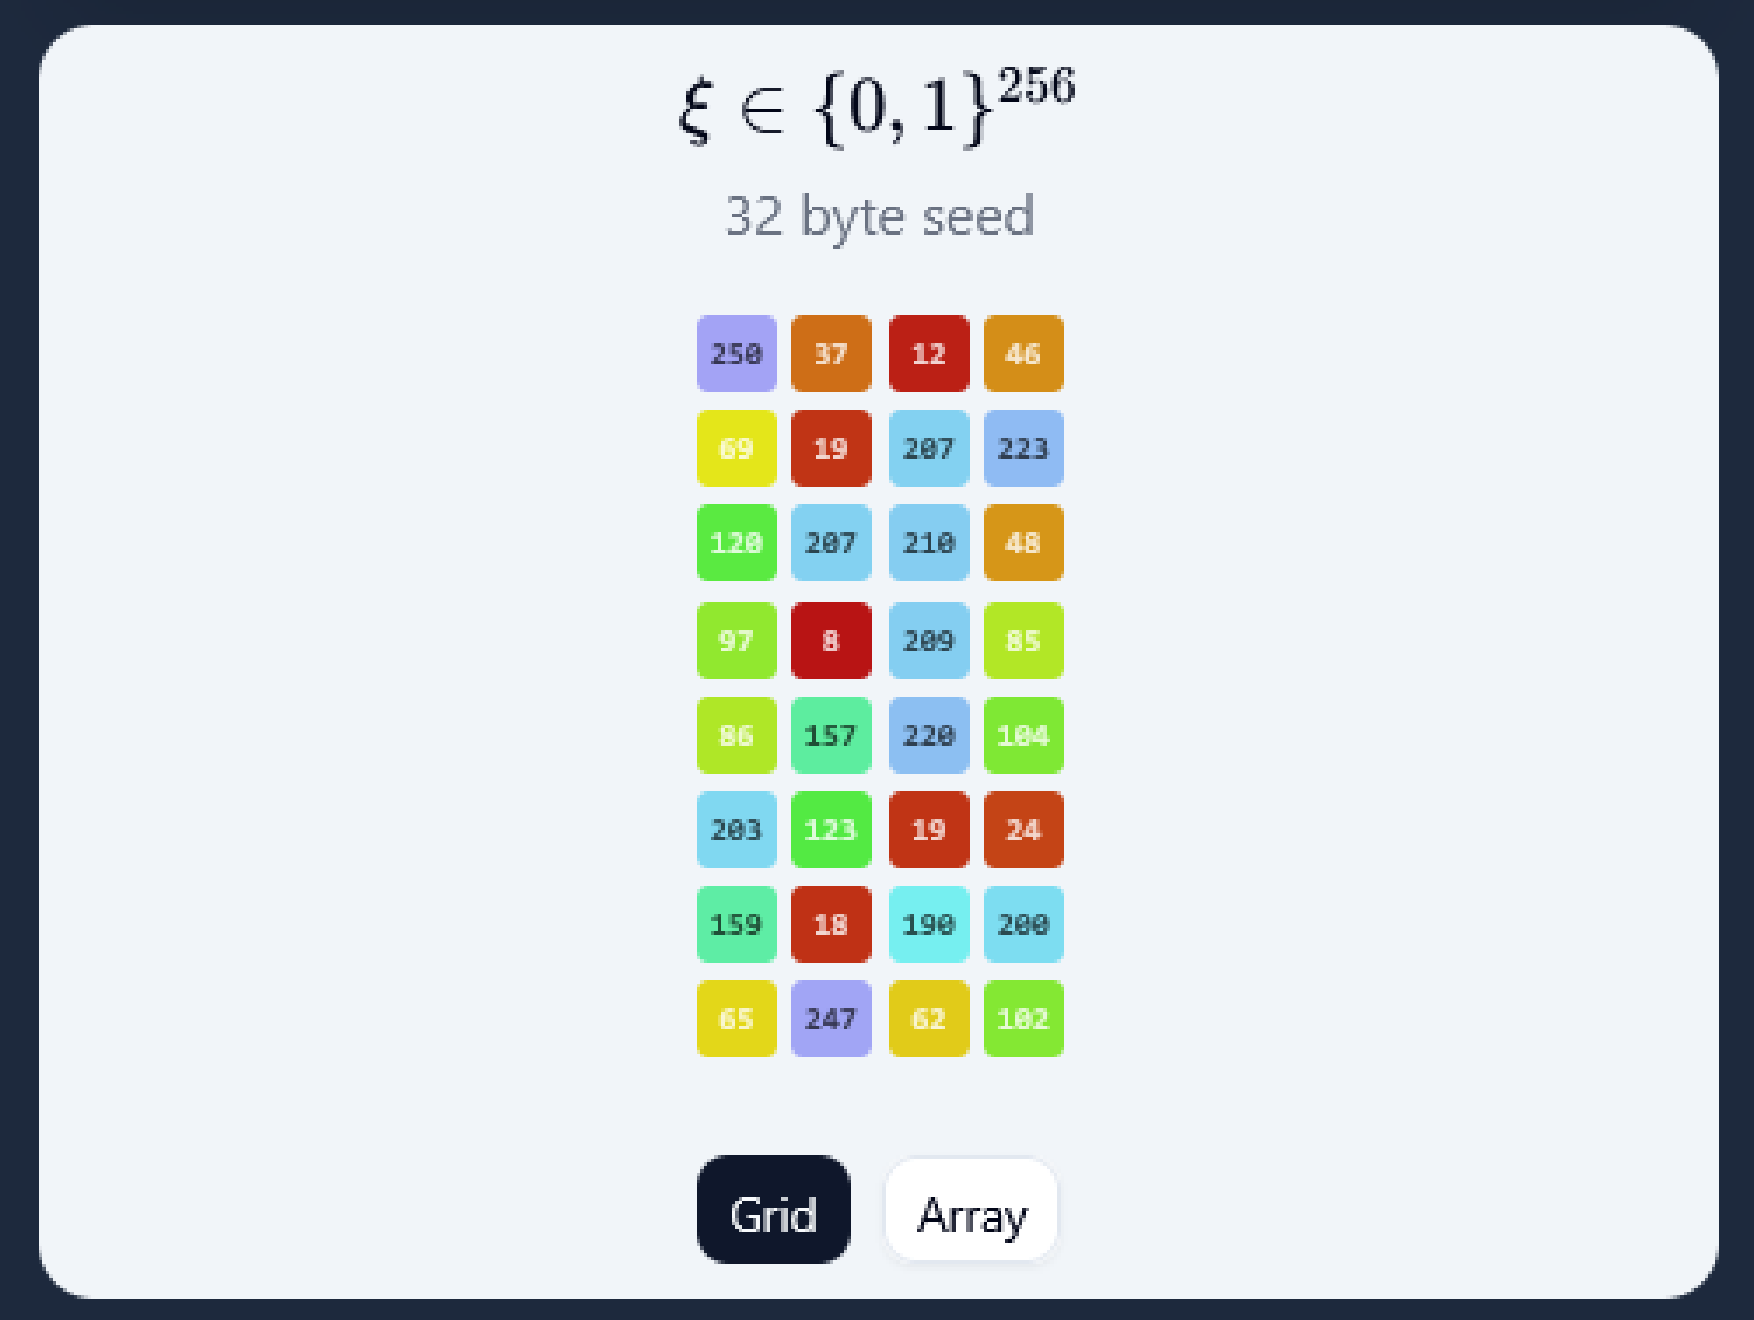
\includegraphics[width=.4\linewidth]{assets/pdfs/sidegrid.pdf}
  \caption{Grid view}
  \label{fig:sub4}
\end{subfigure}%
\begin{subfigure}{.5\textwidth}
  \centering
  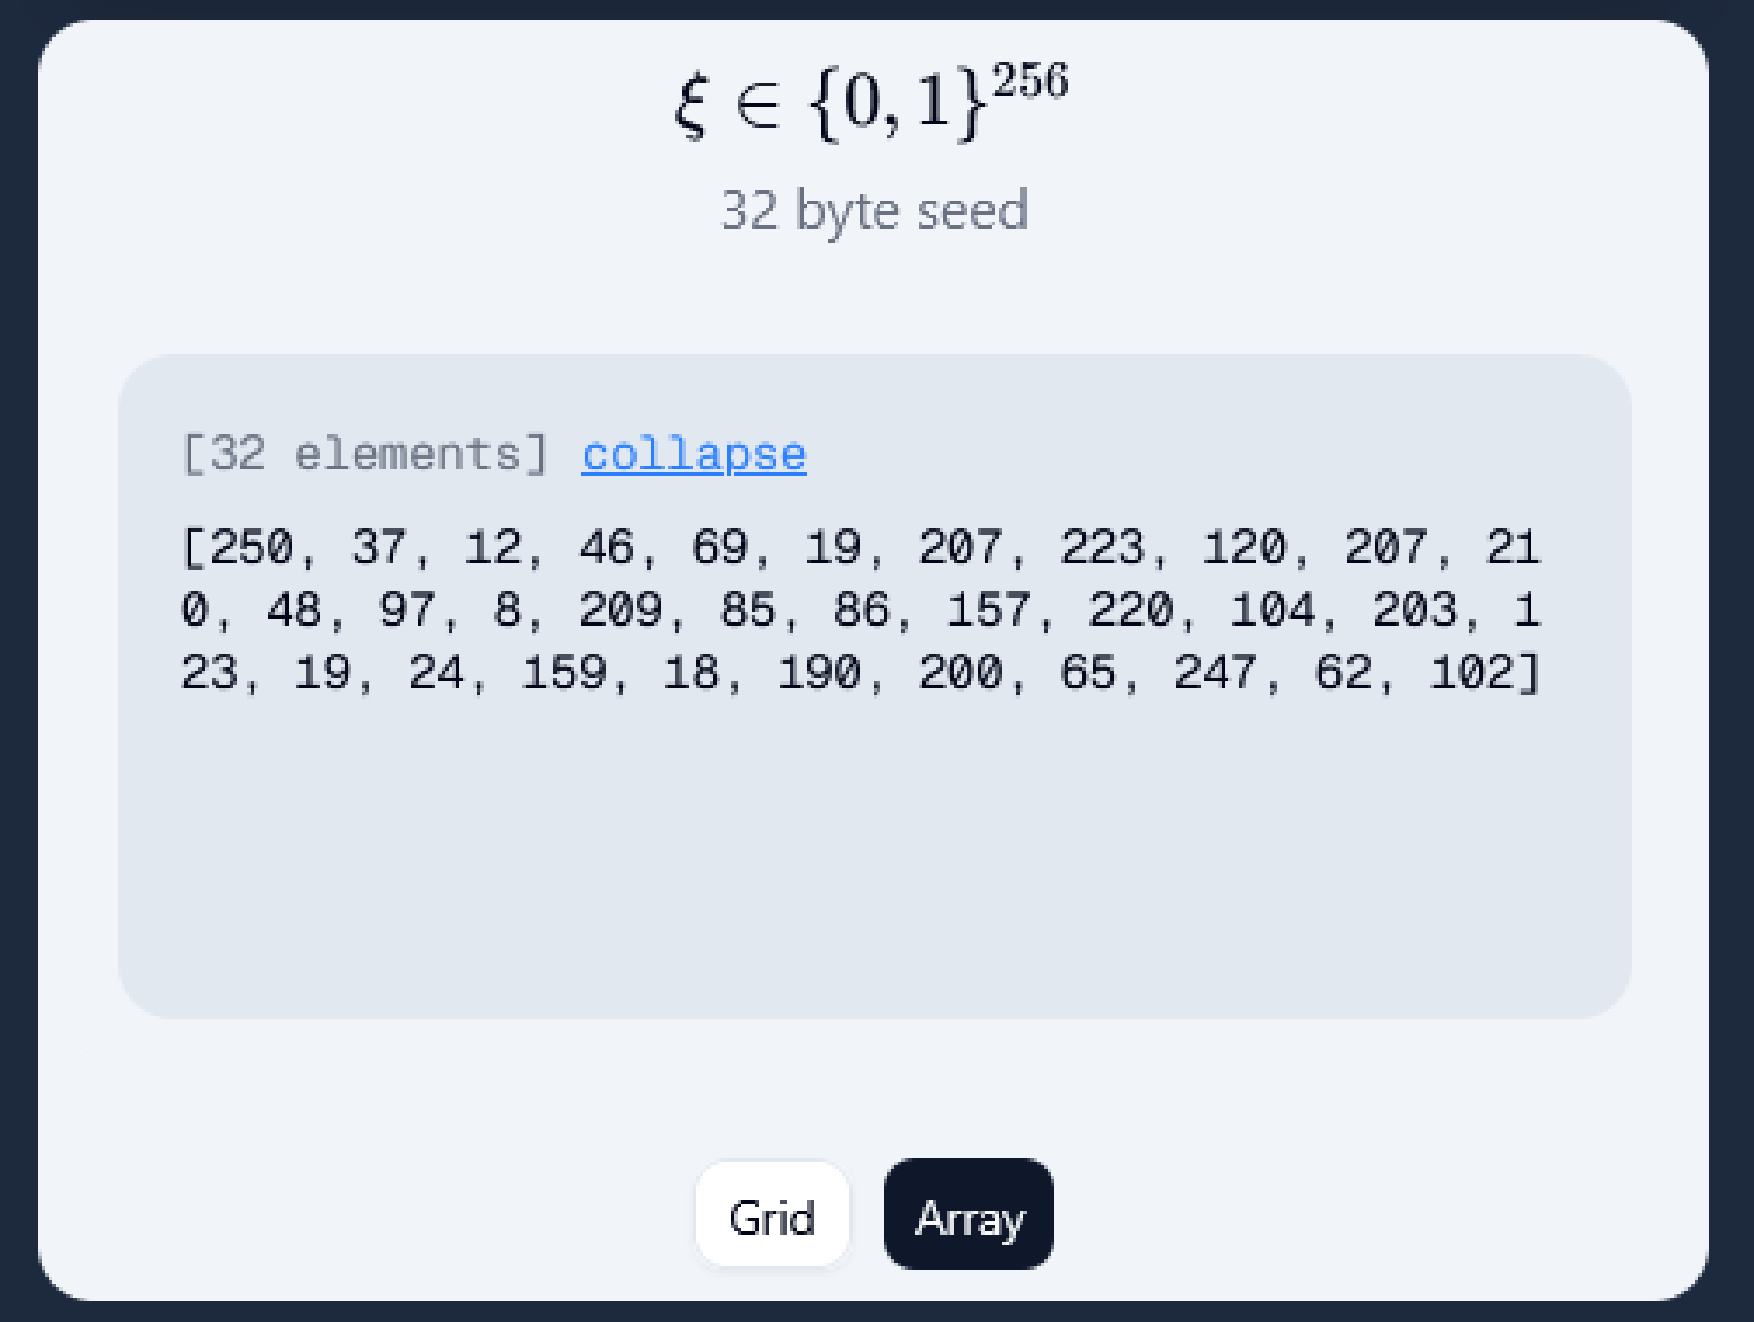
\includegraphics[width=.4\linewidth]{assets/pdfs/sidearray.pdf}
  \caption{Array view}
  \label{fig:sub5}
\end{subfigure}
\caption{Full variables in the side component}
\label{fig:sideview}
\end{figure}

When a function is clicked on, it will lead to a visualization of that function. For example, the internal key generation function seen in Figure~\ref{fig14} (more formally known as ML-DSA.KeyGen\_internal) will show the following:

\begin{figure}[H]
\centering
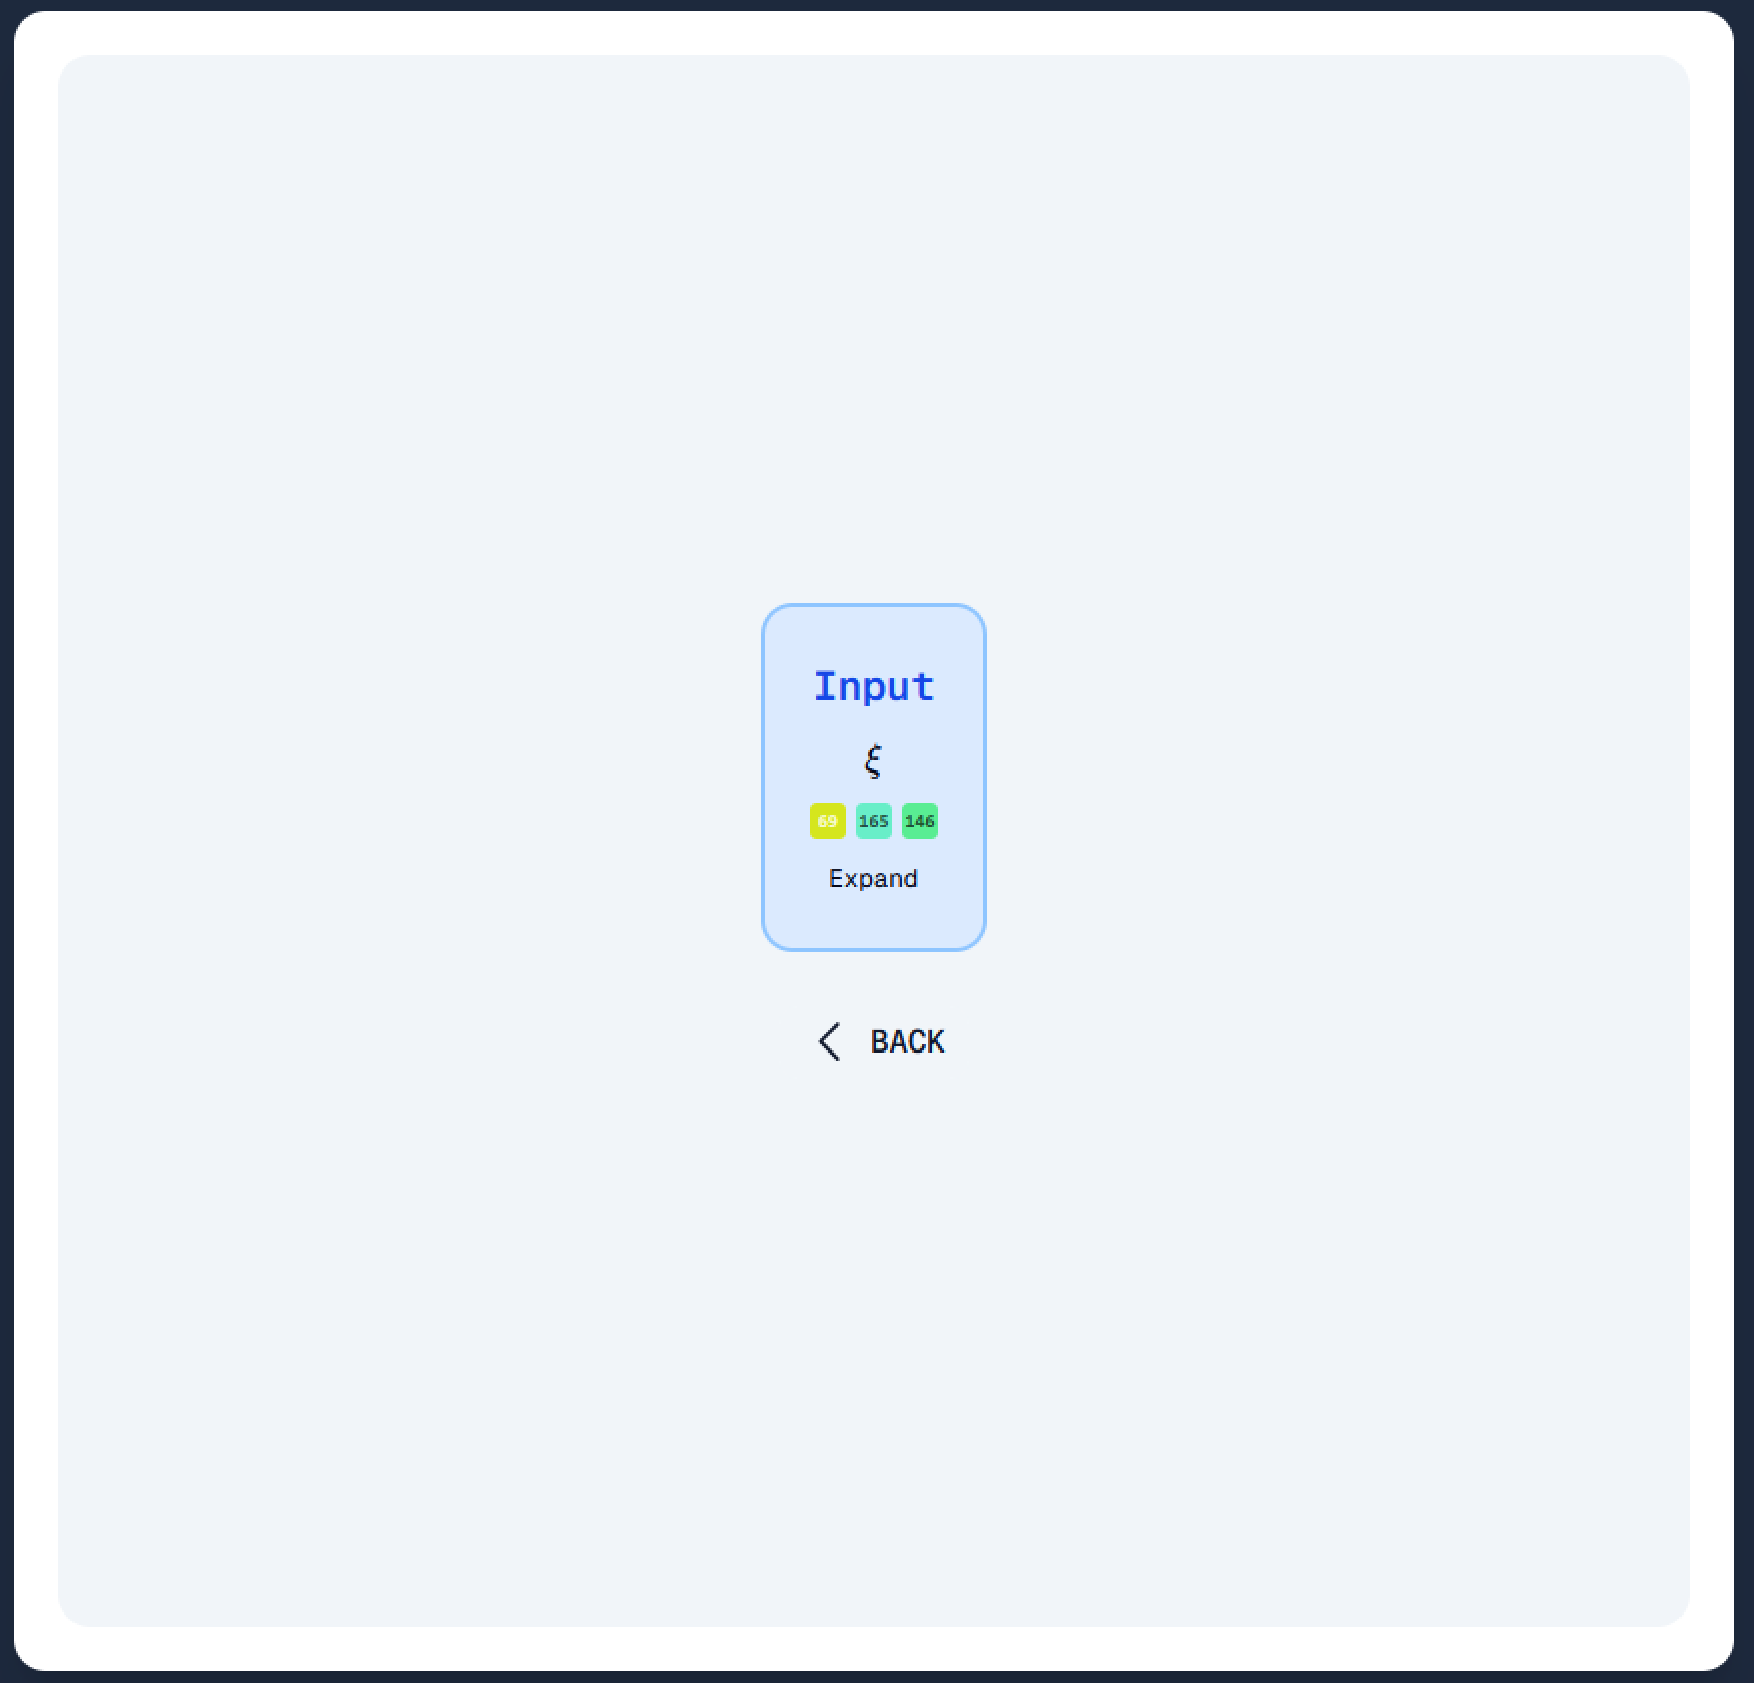
\includegraphics[width=.48\linewidth]{assets/pdfs/default_func.pdf}
\caption{ML-DSA Full Animation Section (Step 1)}
\label{fig16}
\end{figure}

The figure above shows the first step of the function, the input. Subsequent steps can be shown and removed by clicking on the right and left arrows on the lower-right component. Instead of showing the entire function at once, this serves to split the function into more easily followed steps where one part clearly leads to another.

\begin{figure}[H]
\centering

\includegraphics[width=.48\linewidth]{assets/pdfs/step_9.pdf}
\caption{Stepping Component}
\label{fig17}
\end{figure}

\begin{figure}[H]
\centering
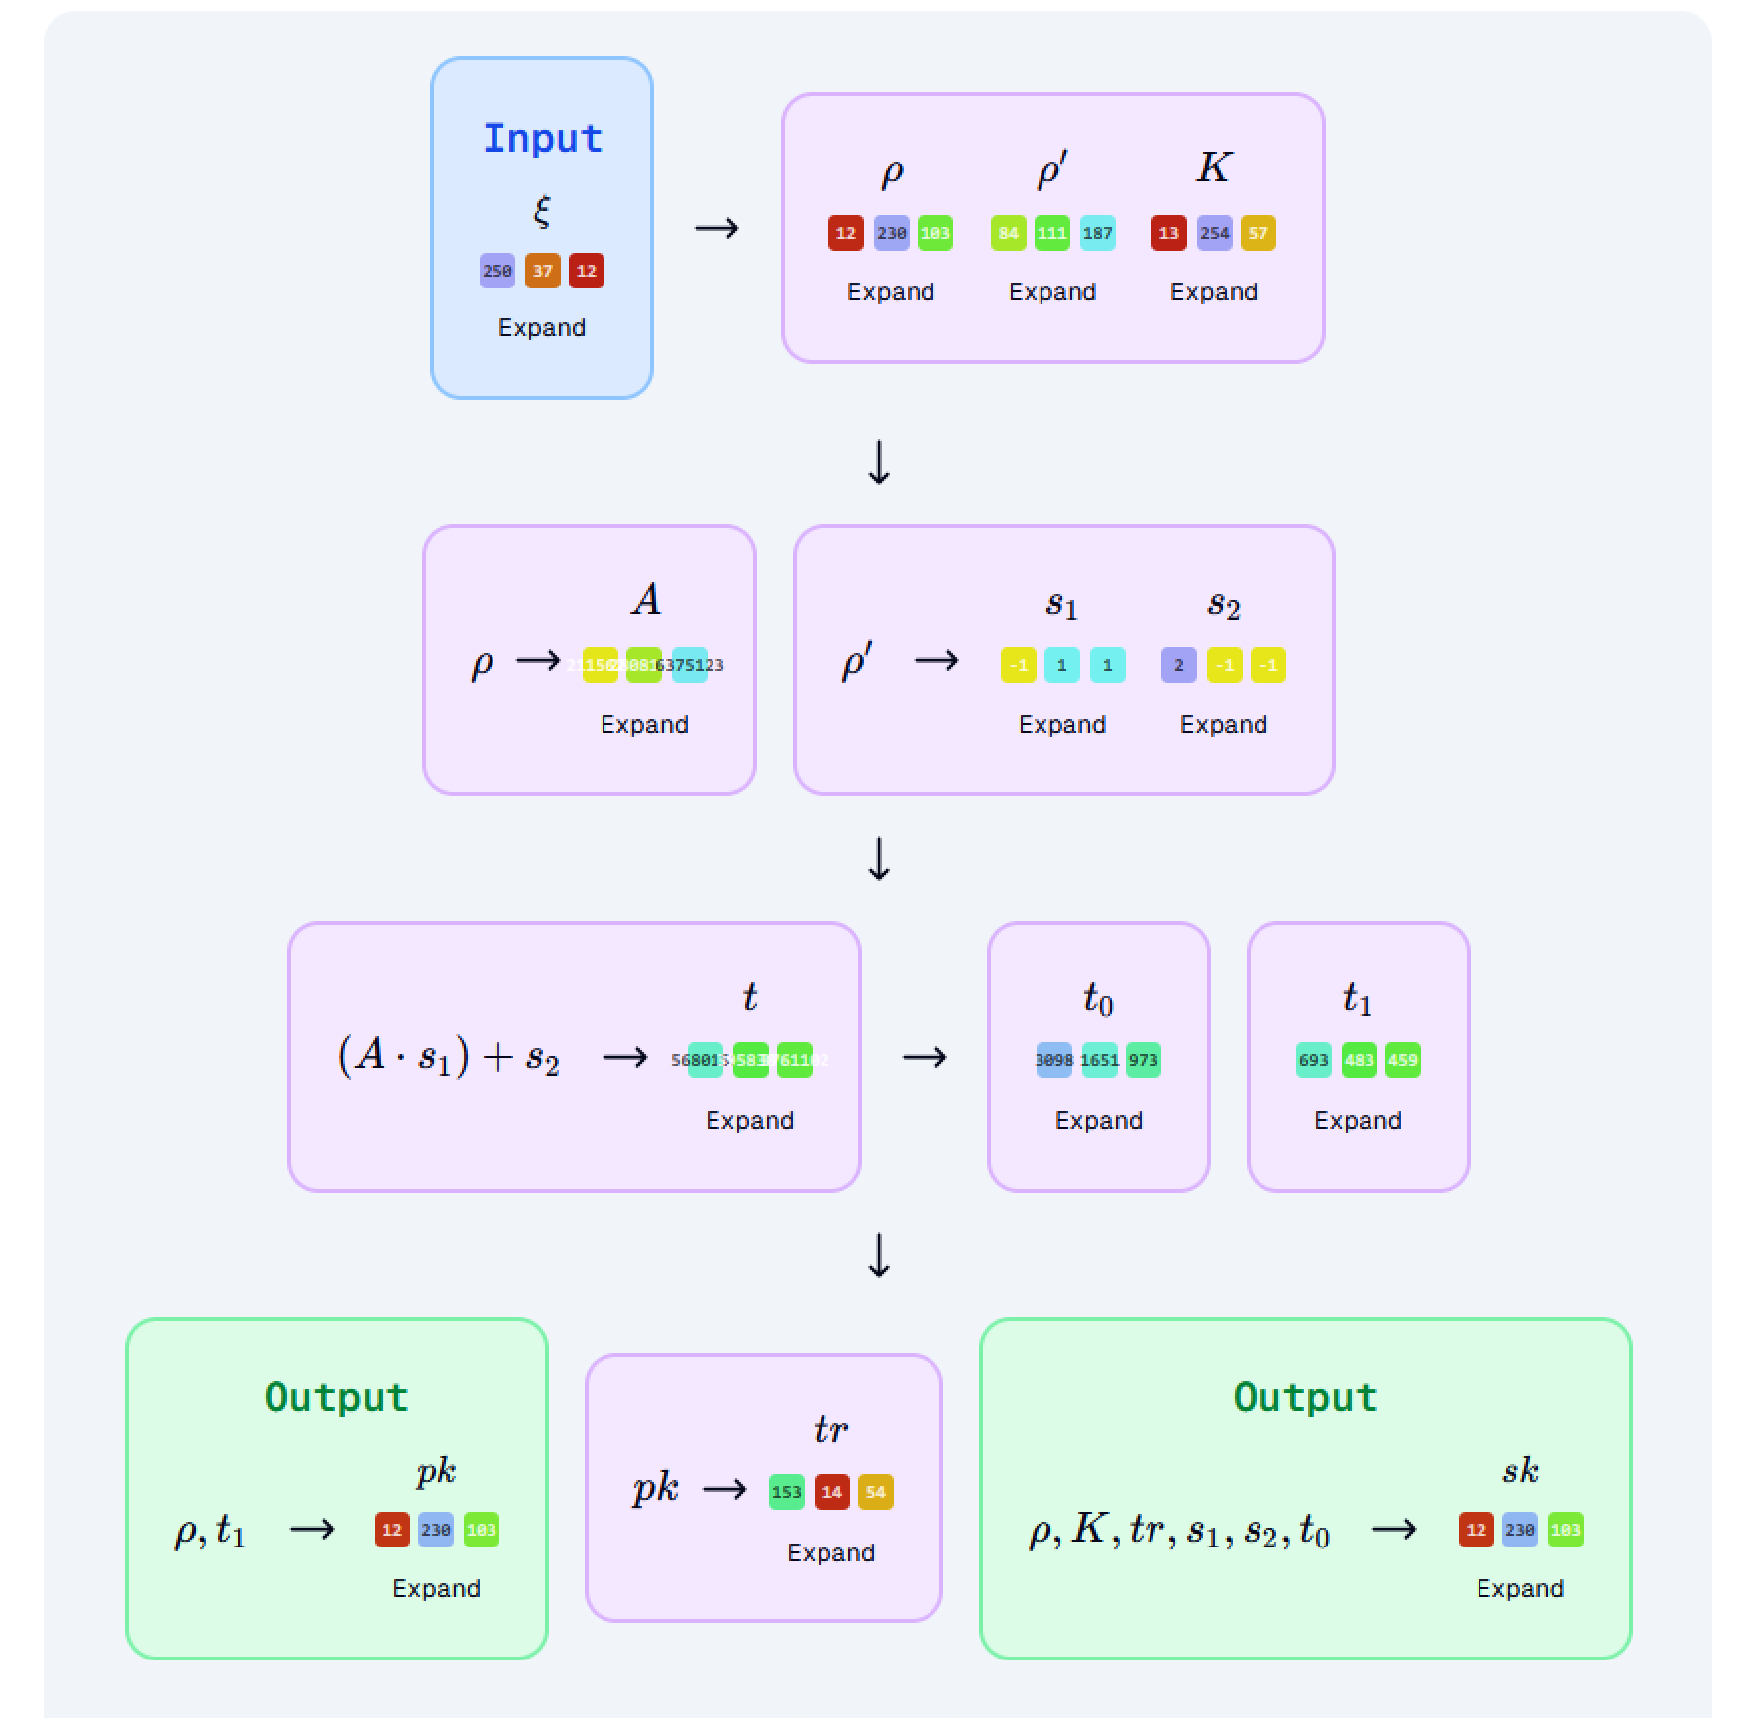
\includegraphics[width=.48\linewidth]{assets/pdfs/keygen_internal_viz.pdf}
\caption{ML-DSA Full Animation Section (Step 9)}
\label{fig18}
\end{figure}

For ML-DSA specifically, there is also a loop function that visualizes each iteration of the valid signature generation loop, elaborating on where and why each specific iteration prior to the last one is invalid.

\begin{figure}[H]
\centering
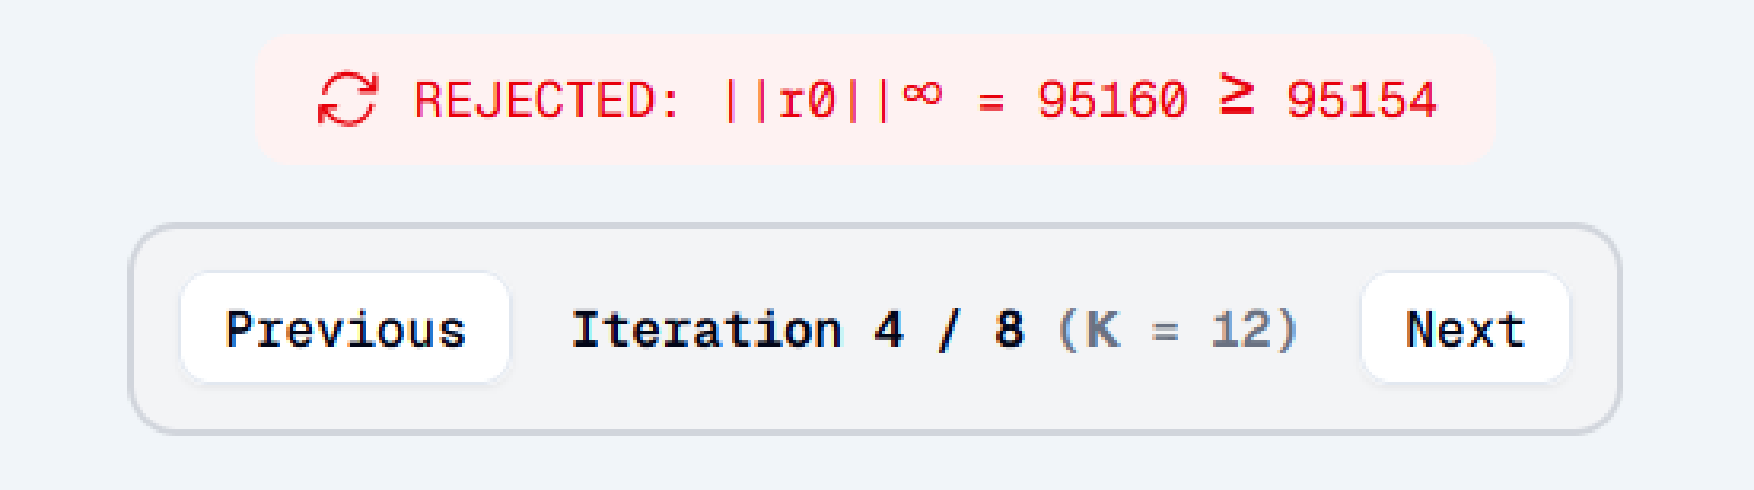
\includegraphics[width=.48\linewidth]{assets/pdfs/loopiteration.pdf}
\caption{Sign Loop Iteration Control}
\label{fig19}
\end{figure}

\subsubsection{LLL and BKZ}
Vector visualization is a very essential concept for gaining proper understanding of linear algebra concepts \cite{15}. This also includes LLL and BKZ algorithms. And so, for both 2D and 3D visualization panels in each modules of LLL and BKZ, we will depict the vectors extracted from the input (the matrix we inserted) as Euclidean vectors within 2D and 3D Cartesian coordinate system. The reason why the Euclidean vectors were chosen to represent the processes as well the inputs of the LLL and BKZ is because both algorithms are obviously lattice reduction algorithms, which operate on the vectors within a Euclidean space. As such, visualizing both algorithms through Euclidean vector representations become a natural choice to show the behavior of lattice bases during the lattice reduction processes. Subprocesses within LLL and BKZ such as the Gram-Schmidt Orthogonalization, basis reduction, and vector swapping (LLL), as well the localized LLLs (BKZ) are involving changes of length, direction, and angles of these vectors. To numerically map the Euclidean Space, the Cartesian coordinate system is implemented, on the basis that lattice basis vectors are naturally represented numerically as coordinates in Euclidean space. Since the LLL and BKZ algorithms operate through geometric transformations of vectors, it could be stated that the Cartesian coordinate system is an intuitive way to visually display the changes of the properties of these vectors. 

Within the Cartesian coordinate system used, whether it is the 2D or the 3D visualization, these vectors are depicted as arrows that are anchored to the origin point of (0,0) in 2D Cartesian coordinate and (0,0,0) in 3D Cartesian coordinate. The reason why the coordinates of (0,0) and (0,0,0) become common origin points of all vectors within the visualization panel is to simplify the observation of geometric properties between basis vectors. Thus, by anchoring all vectors to these common origin points, users can directly compare the orientations and magnitudes of vectors without additional coordinate transformations or positional offsets. Conventionally, how the vectors are visualized in linear algebra and vector geometry in the linear algebra (which also includes lattice reduction algorithms like LLL and BKZ) are as arrows originating from the coordinate origin, which in this case, is (0,0) for 2D visualization and (0,0,0) for 3D visualization. Each arrows has different colouring scheme and is unique in terms of value, as every vectors are unique (as they're linearly independent). No vectors would have more than one arrow that represents them (as they all must be linearly independent). And thus, by representing basis vectors as Euclidean vectors inside Cartesian coordinate systems which all starts from (0,0) as the "anchor point", and with unique colour for each single vector, the users are expected to be able to visually observe how highly non-orthogonal bases gradually transform into shorter and more orthogonal bases throughout the LLL and BKZ algorithms in an easier way. 

Inside the visualization modules for LLL and BKZ, some elements from both algorithms are better visualized, while some others are better shown in textual format. 

\mbox{}
\begin{figure}[htbp]
    \centering
    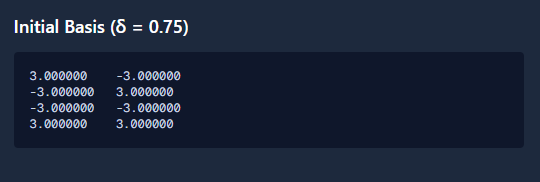
\includegraphics[width=0.7\textwidth]{assets/pics/initial_basis.png}
    \caption{The initial basis panel (LLL)}
    \label{Initial Basis}
\end{figure}
\mbox{}

The whole visualization process begins after the user insert their matrix in the input field, and then clicked "Insert Matrix" button. Within the frontend system, the inserted matrix is parsed into a 2D array, which represents the basis of the inserted matrix. The outer array represents the entire matrix, while the inner array represents the individual basis vectors which are represented by spatial Cartesian coordinates. These basis vectors will be shown as vectors arranged vertically from top to bottom (just like their matrix counterparts) with the first vector is the topmost vector basis.
For the LLL visualization module, the 2D array, alongside with the inserted $\delta$-value will be passed into the runLLL function (which executes a LLL process) and runBKZ function (which executes a BKZ process) in lll.ts and in bkz.ts. For the BKZ visualization module, the 2D array, the $\delta$-value, and the $\beta$-value will be passed into the runBKZ function in bkz.ts, which executes a BKZ process.  

\begin{figure}[htbp]
    \centering
    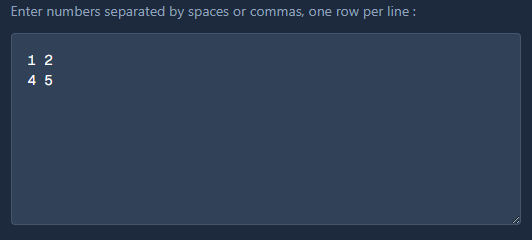
\includegraphics[width=0.7\textwidth]{assets/pics/input_matrix.png}
    \caption{The input matrix}
    \label{input matrix}
\end{figure}
\mbox{}
\begin{figure}[htbp]
    \centering
    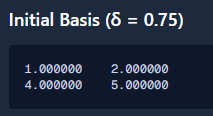
\includegraphics[width=0.7\textwidth]{assets/pics/basisfromtheinputmatrix.png}
    \caption{Basis vectors from the input matrix}
    \label{basis of the matrix}
\end{figure}
\begin{figure}[htbp]
    \centering
    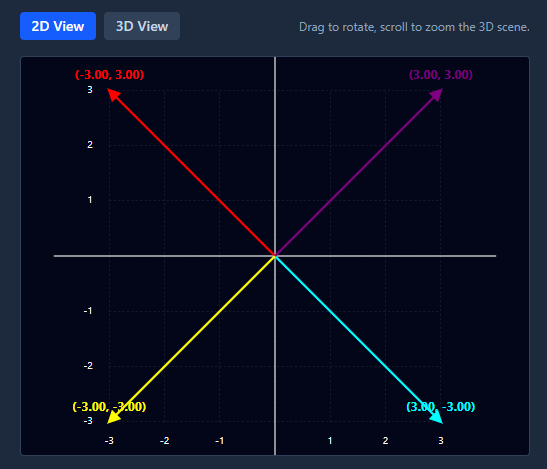
\includegraphics[width=0.7\textwidth]{assets/pics/2Dvisz.png}
    \caption{Basis vectors from the input matrix, represented in the Cartesian coordinate within a Euclidean space}
    \label{cartesian representation}
\end{figure}
\begin{figure}[htbp]
    \centering
    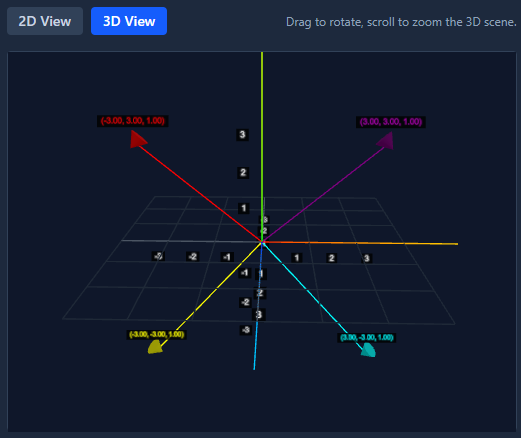
\includegraphics[width=0.7\textwidth]{assets/pics/3Dvisz.png}
    \caption{The 3D version}
    \label{cartesian representation}
\end{figure}
\mbox{}
As what was already stated before, the basis vectors extracted from the input matrix are represented visually as Euclidean vectors inside Cartesian coordinate systems. Thus, each vector is displayed as an arrow originating from the coordinate origin ((0,0) in the 2D visualization or (0,0,0) in the 3D visualization), each one having a unique color, and each one pointing toward the coordinates which represent their numerical values - or the elements of the matrix. For example, the vector $v_1 = (4,5)$ is visualized as an arrow from the origin point of (0,0) toward the point (4,5). Because all vectors are anchored to the origin point, this allows users to observe the length and direction of these vectors, as well the change of them during the reduction process from the beginning until the final output.

The Gram-Schmidt Orthogonalization subprocess would be better off explained through textual explanation in a pop-up window when the user clicks "Show Calculations" button in the "Step and Calculation Details" panel (which we will explain it in the section 4.3.3). At first, the LLL module's frontend source code (lll/page.tsx) would call the runLLL function from the backend source code of lll.ts and inserts the needed parameters - which consist of the basis vectors, the $\delta$-value, and the Boolean flag "true". Within the runLLLL function, it would call the function gramSchmidt and the program would insert the basis vectors to the function and the gramSchmidt function would perform a Gram-Schmidt Orthogonalization to these vectors. The function returns the orthogonalized version of these vectors. Later, the function generateGSOCalculations would be called and then these orthogonalized vectors, alongside the original vectors, are inserted to the generateGSOCalculations function in order to generate a textual display of the mathematical steps behind the Gram-Schmidt Orthogonalization. 

Next, there is vector reduction process, which is shown in the form of a textual explanation of its calculation steps in a pop-up window. How the textual explanations of the calculations behind the vector reduction and vector swap processes are displayed is roughly similar to the Gram-Schmidt process explanation. When the frontend called runLLL function from the backend source code of lll.ts, after performing Gram-Schmidt Orthonalization and other conditions for the vector reduction to be performed, it would call the function vectorSubtract - which as its name suggests, performs a vector size reduction process. The output produced by vectorSubtract, together with the previous vector and the currently examined vector would then be inserted into a function named generateReduceCalculations in order to generate a textual display of the mathematical steps behind the vector size reduction process.

Then, if the current basis doesn't satisfy the Lovasz Condition, it wouldn't only triggered a vector reduction, but also the vector swap after the vector reduction. The currently examined vector would has its index getting switched with the index of the previous vector. Later, the function of generateSwapCalculations would be executed, which generates a textual display of the mathematical steps behind the vector swap process. 

And then, there is Lovasz Condition. It is depicted as a status panel of two states ("Satisfied" and "Not Satisfied"). Unlike with the usual mechanism of Lovasz Condition checking, for convenience reasons, the Lovasz Condition status is continously being displayed even when the current process isn't the Lovasz Condition checking as in the common LLL algorithm. This is achieved through the addition of the the function computeLovaszStatus in the app/lll/page.tsx functions to continously checking the Lovasz Condition status in order to keep the Lovasz Status panel has a status at one time, from the first step of the process until the final step. The regular Lovasz Condition checker - the function lovaszCondition in the backend code - was created to perform Lovasz Condition checking only after the currently examined vector has been reduced. Of course, there is a risk of these two Lovasz Condition checkers would have two different answers at the same time, but this risk had been eliminated by employing them into separate responsibilities. The computeLovaszStatus rechecks the Lovasz Status condition based on the existing data gained from LLL execution by the backend.

And finally, the SVP. The SVP is computed throughout each of the BKZ iterations, and in LLL, computed from the vectors from the final output. However, Latviz would only show the SVP at the final step of both algorithms, and it is displayed within a dedicated panel in the LLL and BKZ modules.
